\def\arxiv{0}
\def\cogsci{1}

\if\arxiv 1
\documentclass[twocolumn,a4paper,superscriptaddress,nofootinbib]{revtex4}
\fi

\if\cogsci 1
\documentclass[a4paper]{article}
\usepackage[a4paper,top=2.5cm,bottom=2.5cm,left=2.5cm,right=2.5cm]{geometry}
\usepackage[natbibapa]{apacite}
\usepackage{times}
\usepackage{xcolor}
\fi

% commands
\definecolor{green2}{rgb}{0.55, 0.71, 0.0}
\newcommand{\tobo}[1]{{\color{red} TOBO: #1}}
\newcommand{\tsn}[1]{{\color{blue} TSN: #1}}
\newcommand{\add}[1]{{\color{green2} Add: #1}}

\newcommand{\re}[1]{{\color{brown} RE: #1}}
\newenvironment{robin}{\smallskip \noindent \color{red!10!green!50!blue}}{\color{black}\smallskip}

% Packages
\usepackage[caption=false]{subfig}  % needed for compatibility btw revtex and captions
\usepackage{dcolumn}   % needed for some tables
\usepackage{graphicx}
\usepackage{titlesec}
\usepackage{amsmath}
\usepackage{amssymb}
\usepackage{amsthm}
  \newtheorem{theorem}{Theorem}
  \newtheorem{lemma}[theorem]{Lemma}
  \newtheorem{definition}[theorem]{Definition}
\usepackage{tikz}
\usepackage[utf8]{inputenc} % for at få danske karakterer. Kræver at alle bruger en editor som understøtter utf8.
\usepackage{hyperref}
\usepackage{soul} % for strikethrough

% Macros
\definecolor{mygreen}{rgb}{0,0.6,0}
\newcommand{\at}{\makeatletter @\makeatother}
\newcommand{\tmin}{t_{\min}}
\newcommand{\tmax}{t_{\max}}

% Style parameters
\if\arxiv 1 
\setlength{\parskip}{0pt}
\setlength{\tabcolsep}{6pt}
\setlength{\arraycolsep}{2pt}
\titlespacing*{\section}
{0pt}{2ex}{1ex}
\titlespacing*{\subsection}
{0pt}{2ex}{1ex}
\titlespacing*{\subsubsection}
{0pt}{2ex}{1ex}
\fi

\graphicspath{{../plots/}{../images/}}


\begin{document}
\if\cogsci 1
\setlength{\baselineskip}{1.44\baselineskip} % empirically this seems to match MS Word's idea of 1.5 line spacing % TSN: I found \linespread{1.25} to be Word's 1.5 line spacing, might be the same in effect.
% TOBO: 1.44\baselineskip is from the Danish National Research Councils and what they use to get the same effect in Latex as 1.5 line spacing in Word. Where did you find the suggestion to use \linespread{1.25}?
\fi


\title{The Curse of Shared Knowledge: Recursive Belief Reasoning in a Coordination Game with Imperfect Information}
\if\arxiv 1
\author{Thomas Bolander}
\affiliation{Department of Applied Mathematics and Computer Science, Technical University of Denmark, Richard Petersens Plads, building 324, DK-2800 Lyngby, Denmark}
\author{Robin Engelhardt}
\author{Thomas S. Nicolet}
\affiliation{Center for Information and Bubble Studies, Department of Communication, University of Copenhagen, Karen Blixens Plads 8, DK-2300 Copenhagen S.}
\fi

\if\cogsci 1
\author{Thomas Bolander, Robin Engelhardt, Thomas S. Nicolet}
\fi



%\significancestatement{Anybody who has been caught up in a sidewalk dance knows that human coordination without common knowledge is prone to failure. When common knowledge cannot be obtained, humans routinely act upon their private knowledge, or upon their shared reasoning about other minds. While we know much about human limits to such higher-order belief reasoning, little is known about at which point, and under which circumstances, shared knowledge becomes effectively indistinguishable from common knowledge. We investigate this question with a novel recursive coordination game with imperfect information, and show that people consistently act as if they have common knowledge about a fact, even in situations where they share only the shallowest levels of their state of mind.}

\maketitle

\begin{abstract}
Common knowledge is a necessary condition for safe group coordination. When common knowledge cannot be obtained, humans are forced to rely on shared knowledge only.
%humans rely on their ability to identify shared knowledge to distinguish who knows what.
%When common knowledge can not be obtained, humans routinely use their ability to attribute beliefs and intentions \tobo{What does intentions have to do with it? Next sentence also says "*such* shared knowledge attributions", which in principle is neither about beliefs nor intentions.} \tsn {Maybe I misunderstand, but intentions are related due to the fact that coordination relies on being able to correctly attribute (predict) the intentions of others. But I find another issue: It might imply that people *only* attribute beliefs to others when common knowledge cannot be obtained. But every social action involves belief attribution (or attributing some mental state to others). So, could word it as something like "When common knowledge cannot be obtained, humans rely on their ability to identify shared knowledge to distinguish between who knows what" }  in order to infer what is known. 
But shared knowledge is limited in depth and therefore prone to coordination failures. %because any finite-order knowledge attribution allows for an even higher order attribution that may change what is known by whom. 
In three separate experiments, we investigate to which degree human participants (N=802) are able to recognize the difference between common knowledge and nth-order shared knowledge. We have designed a two-person coordination game with imperfect information that is able to cast the recursive game structure and higher-order uncertainties into a simple, everyday-like setting. In the game, successful coordination to achieve the highest payoff requires a specific fact to be common knowledge among the participants. However, this is impossible to achieve in the game, the fact can at most be nth-order shared knowledge for some n.
%only nth-order shared knowledge can be achieved for varying values of n.
  Our results show that already from quite shallow depths of shared knowledge (small values of n), the participants act as if they had common knowledge, and express similar certainty in their actions as if they had. We call this phenomenon `the curse of shared knowledge'. It occurs in spite of participants suffering huge payoff penalties when falsely assuming that coordination, and hence common knowledge, is guaranteed.
  %\tsn{Måske korte lidt ned, eller hive lidt i land? Synes ikke vi konkluderer for stærkt her, udover måske "express certainty", som måske altid er lidt svært at rigtigt vide.} \add{
  We conjecture that this is either due to participants' inability to distinguish between higher-order shared and common knowledge, or the implicit assumption that their co-player cannot.
  
%express to be completely certain about being coordinated and achieving the highest payoff,  
% express to be as certain that they are coordinated and will achieve the highest payoff as if they indeed had common knowledge. 
%Despite this, our results show that participants behave as if they had common knowledge, and for sufficiently large values of n, they claim to  
% in self-assessing the certainty of receiving the 
%their actions
%claim their actions to be as certain as if they had common knowledge. 
%It is impossible to achieve common knowl
%
%Our results show that participants have a very hard time accepting the fact that common knowledge is not reducible to shared knowledge.\tobo{Maybe too strong? Do our results really show that? They behave as if having common knowledge, but they might still be able to distinguish common knowledge achieved via public announcements from what they have in this game.} Instead, participants try to coordinate even at quite shallow depths of shared knowledge and in spite of huge payoff penalties. \tsn{With regards to Tobo's comments consider the following alternative: "Our results show that participants try to coordinate when the levels of shared knowledge gets sufficiently high. In other words, our participants behave as if they have common knowledge about facts that are only shared knowledge, and collectively suffer huge payoff penalties as a result."} \re{Yes too strong, i guess. Proposal, taget fra TOBO: "Our results show that participants behave as if they had common knowledge. Participants also claim to be certain about their actions as if they had common knowledge, even when common knowledge is not obtainable."}
\end{abstract}


\section{Introduction}
Anybody who has been caught up in a sidewalk dance knows that human coordination without common knowledge about each other's intentions is prone to failure. Thus, cooperating humans have evolved techniques by which to create common knowledge in practice, such as eye contact, conventions, and broadcasted messages. When common knowledge cannot be obtained, humans routinely act upon their private knowledge, or upon their shared reasoning about other minds. While we know much about human limits to such higher-order belief reasoning, little is known about at which point, and under which circumstances, shared knowledge becomes effectively indistinguishable from common knowledge. We investigate this question with a novel recursive coordination game with imperfect information, and show that people consistently act as if they have common knowledge about a fact, even in situations where they share only the shallowest levels of their state of mind. 

Successful group coordination requires complementary choices among group members, which, in turn, requires communication of beliefs and intentions in such a way that they become common knowledge~\citep{fagin1995reasoning}. A fact is said to be \textit{common knowledge} if everyone knows it, and everyone knows everyone knows it, and everyone knows everyone knows everyone knows it, and so on, ad infinitum~\citep{lewis1969convention, clark1981definite, schelling1980strategy, aumann1976agreeing}. If the premise of ``everyone knows'' is not infinitely nested, but only nested to finite depth, we instead have \emph{shared knowledge}. If there is no nested knowledge about knowledge at all and not everyone necessarily knows the fact, we have \emph{private knowledge}.

Let us illustrate the difference between these notions with an example. Two friends, Agnes and Bertram, are taking different trekking routes on the same mountain, and have agreed to meet at the top. 
%In the morning they agree that if the weather gets bad, they will go back down and sleep in the mountain hut at the base. Otherwise, they strongly prefer to stay overnight at the top. 
The equipment essential for an overnight stay at the top has been divided between their backpacks, so it's crucial for their safety that they meet there before it gets dark. 
%. It is therefore crucial that if one of them decides to go to the top, the other one does the same. 
On the way to the top, they both observe bad weather approaching, which makes it safer to go back to the base. However, they are both uncertain about whether the other person has seen the bad weather, so they cannot expect the other person to necessarily go to the base. The most dangerous situation is if one of them goes to the base and the other goes to the top, since then one of them is left at the top without the necessary equipment to stay there for the night. 

At this point they both know the fact that ``bad weather approaches'', but don't know whether the other knows. In this situation, we would say that Agnes and Bertram both have \emph{private knowledge} that bad weather is approaching, and since they both know it, it is also \emph{shared knowledge} between them. More generally, a fact is \emph{private knowledge} in a group of agents if some non-empty subset of the agents know the fact. For the special case where everybody in the group knows it, we say that there is \emph{shared knowledge to depth one} (or \emph{first-order shared knowledge}) of the fact~\citep{clark1981definite}. The exact border between what is considered private and shared knowledge vary significantly between different papers. Some consider the case where everybody knows a fact to still only be private knowledge, and that for it to be shared knowledge, at least one agent also needs to know that they all know. The notion of shared knowledge we use in this paper, where shared knowledge only requires that everybody knows, is the most standard in (epistemic) logic. Formal definitions of private, shared and common knowledge as well as a more detailed discussion of our choice of conventions can be found in the Supplementary Material.\footnote{Supplementary Material is accessible at \url{http://www2.compute.dtu.dk/\~tobo/cd_sm.pdf}.}

Since Agnes doesn't know whether Bertram knows about the bad weather, she would like to warn him and suggest to meet back at the base. So she sends a text message: ``Bad weather approaching. Let's meet at base.'' However, due to the unstable mobile network signals, she is not certain that the message will go through. Therefore she asks Bertram to confirm that he received the  message. A few minutes later, she receives his confirmation. At this point it has become \emph{shared knowledge to depth two} (or \emph{second-order shared knowledge}) that bad weather is approaching: He knows that she knows, since he received her message, and she knows that he knows, because she received his confirmation. To have \emph{shared knowledge to depth three} (\emph{third-order shared knowledge}), it would additionally be required that A) she knows that he knows that she knows, and B) that he knows that she knows that he knows. In fact, A already holds, since he confirmed receiving her message. However, B doesn't hold, since he will be uncertain about whether his confirmation was successfully received. Thus we have asymmetry in the level of knowledge of the two agents. If he also asks her to confirm his message, and he receives such a confirmation, then of course he will get to know that she knows that he knows. Then there will be shared knowledge to depth three. However, there will still be a (higher-order) knowledge asymmetry, since Agnes can't be certain that the last message was received.

How many messages back and forth does it take for Agnes and Bertram to coordinate going back to the base? At first it might seem that it is sufficient for both of them to know that at least one of them plans to go to the base. However, that is not so. After the first message has been received, both know that Agnes plans to go to the base, but she is still uncertain whether he knows. And if he doesn't, she might risk leaving him alone at the top. So shared knowledge to depth one is clearly not sufficient. Even shared knowledge to depth two is not sufficient. After he has confirmed receiving her original message, from his perspective it is still entirely possible that she doesn't know that he knows, and hence, she might decide to go to the top to not leave him alone up there. And in this case, he also has to go to the top in order not to leave \emph{her} alone up there. This argument can be generalised to prove that even $n$th-order shared knowledge for any arbitrary large $n$ is insufficient for safe coordination.\footnote{To derive a contradiction, suppose $n$th-order shared knowledge for some $n$ is sufficient to make it safe to go to the base, in the sense of guaranteeing that the other person will also go there. This implies that the successful delivery of the $n$th message is sufficient to guarantee meeting at the base. There must then exist a smallest number $n_0$ such that the successful delivery of the $n_0$th message is sufficient to guarantee meeting at the base. Since $n_0$ is the smallest such number, the successful delivery of the $(n_0-1)$st message is not sufficient to guarantee meeting at the base. Now note that at the moment when the $n_0$th message has been successfully delivered, the sender of this message is still uncertain about whether it was actually received, and hence the sender is only certain that the first $n_0-1$ messages has been successfully delivered.  In other words, the sender of the $n_0$th message considers it possible---even after the successful delivery of the message---that only the first $n_0-1$ messages were successfully delivered, in which case it is \emph{not} safe to go to the base. Hence that person will after having sent the $n_0$th message stil consider it unsafe to go to the base, and will choose to go to the top. This is a contradiction, completing the proof. This proof is stated in rather informal terms, but can be turned into a formal, mathematical proof~\citep{fagin1995reasoning}. The example here is in fact modelled after the coordinated attack problem studied extensively in that book, where it is also used to illustrate that common knowledge is a necessary condition for coordination.}  The consequence is that no finite number of messages successfully delivered will guarantee that Agnes and Bertram manage to meet at the base. In order to guarantee meeting at the base, they would need to have shared $n$th-order knowledge for \emph{all} $n$. Shared $n$th-order knowledge of some fact for all $n$ is called  \emph{common knowledge} of the fact (see again the Supplementary Material for a more formal definition). The essence of the argument is that any  
%\add{This is highly intuitive, but the fact remains that any 
plan for Agnes and Bertram to coordinate without common knowledge would leave one stranded at the top in the case of a faulty signal at a critical point in their communication.
%}

In practice, shouldn't it be possible to coordinate meeting at the base after one or two messages being sent back and forth? It is likely that this is what Agnes and Bertram would attempt, at least. The question is whether they are fully aware of the risk of miscoordination in this case? After Agnes has sent the message and Bertram has successfully confirmed receiving it, are they aware that the content of the message is still not common knowledge, and that they still risk miscoordination? Or do they now believe it completely safe to go to the base? The questions here are whether A) they can distinguish between the case of $n$th-order shared knowledge and common knowledge, and whether B) they would act differently in the case of common knowledge than in the case of $n$th-order shared knowledge for some suitable large $n$. 
% as if they have common knowledge despite only having $n$th-order shared knowledge.    


% Isn't it a purely mathematical problem with no practical implications for humans trying to coordinate their actions? One of the main goals of this paper is to argue that the answer to both questions is no. \tsn{Skal vi ændre formuleringen så vi ikke direkte påstår det har praktiske implikationer ift mennesker, men mere beskriver at det har konsekvenser i det omfang sådanne problematiske epistemiske strukturer findes, selvom (eller specielt derfor), at vi ikke kan indse at de er problematiske (som vores forsøg viser, og som er tydeligt når selv i mountrain-trekking eksemplet er mange kritiske)} 
%In order to make that argument, 
We have designed a coordination game that has a similar underlying mathematical structure as this trekking example, but cast in a simpler setting, where the higher-order uncertainty is established already when the game is initialised and not, as above, through a series of message passings. In this game, our experiments show that human players indeed try to coordinate on the preferred outcome even when only having low orders of shared knowledge (corresponding to trying to meet at the base after only a few message passings in the trekking example). However, this often results in severe cases of miscoordination with high penalty, corresponding to the situation in the trekking example where one of the trekkers would leave the other at the top without the necessary equipment. In our game, the answer to B above is ``no'': Most players definitely act as if they have common knowledge, even though they don't. They play strategies that would have given them the highest payoff if they had had common knowledge, but since they don't, they end up with payoffs that are significantly lower than what they could have received if they had explicitly distinguished the common knowledge situation from the $n$th-order shared knowledge situation. One might however still speculate that this is a 
%Despite this not leading to the game-theoretically optimal strategy, we might speculate that it is nevertheless a 
conscious choice of strategy, and that the players are nevertheless aware that they don't have common knowledge. However, through follow-up questions and interviews, it seems that the answer to A is also ``no'': Players claim they have common knowledge and that coordination is guaranteed, even when they only have low-order shared knowledge.     

We originally developed the game to illustrate how the difference between shared and common knowledge can have a real impact on human behaviour and strategic reasoning. Humans generally find the concept of common knowledge hard to grasp, and even harder to grasp the practical relevance of, due to the unbounded nesting of knowledge.  The game we developed intends to make it clear that human intuitions about common knowledge can be misleading and may have costly consequences.

\section{The curse of shared knowledge}
Reasoning about the knowledge of others, their reasoning about you, and your reasoning about their reasoning, and so on, is famous in cognitive science for its presumed computational intractability~\citep{van2018parameterized,bolander2023parameterized}. Because of this, coordinating species typically use heuristic shortcuts in order to reduce complex shared knowledge states, such as joint perceptual cues and broadcasted signals~\citep{milgrom1981axiomatic, clark1996using, bradbury1998principles}. Humans may obtain common knowledge via mutually accessible first-order sensory experiences~\citep{tomasello1995joint, lorini2005establishing, bolander2015announcements, gintis2010rationality}, eye contact~\citep{friedell1969structure}, public rituals and conventions~\citep{lewis1969convention}, or salient focal points~\citep{schelling1957bargaining}. What most prominently is believed to distinguish human coordination from other animals, however, is the enormous flexibility by which humans can imagine and articulate the mental states of their peers~\citep{tooby2010groups, harari2014sapiens}. The abilities to blush, to tell jokes, and to write novels testify that humans readily attribute \textit{higher-order} beliefs, intentions, and reasoning capabilities to other people, such as thinking explicitly about the mental states of others who think about the thoughts and beliefs of others and so on---while at the same time appreciating that those thoughts and beliefs can differ from each other and from reality. Such higher-order cognition has seen substantial scientific attention, and has brought about various technical terms such as ``Theory of Mind'' (ToM)~\citep{premack1978does}, ``mentalizing''~\citep{frith2003development}, ``mind reading''~\citep{vogeley2001mind, apperly2010mindreaders}, %``mental models''~\citep{johnson1983mental},
``mind perception''~\citep{gray2011distortions}, ``perspective taking'', and ``social intelligence''~\citep{baron1999social}, which often are used interchangeably for studying the cognitive mechanisms of shared knowledge, but sometimes focus on slightly different ideas and associated meanings~\citep{schaafsma2015deconstructing}, depending on the field of investigation.

Looking at the ToM-literature, conclusions about human belief reasoning abilities are rather heterogeneous~\citep{apperly2009humans, saxe2013theory}: Human reasoning about the reasoning processes of other humans is limited~\citep{premack1978does, gopnik1988children, stahl1995players, nagel1995unraveling, hedden2002you, keysar2003limits, pinker2003language}, contextual, and possibly domain specific~\citep{leslie1992domain, saxe2009theory, heyes2014submentalizing}. Three-year-old children tend to fail in the well-known first-order false belief tasks by falsely assuming that their private information is shared by others, while second-order false belief tasks are mastered around ages 5-7~\citep{perner1985john, sullivan1994preschoolers}. Adults may reliably master up to four orders~\citep{kinderman1998theory}, but still have difficulties ignoring the private information they possess when assessing the beliefs of others, resulting in a \textit{curse of knowledge} bias which can compromise their ability to make predictions about other people’s beliefs and actions~\citep{camerer1989curse, birch2007curse}. When the nested mental states represent a succession of different people, such as ``Alice thinks that Bob thinks that Carol is contemplating the idea that David is thinking about Evelyn'', we have less problems following along\footnote{Especially when those successions of mental states are qualified by psychological attribute words such as `Alice thinks that Bob is mistakenly worrying that Carol is offended by misunderstanding something Dave had said to Evelyn'.~\citep{academian2019unrolling}.
} than when the nested mental states are successions of the same people over and over again, and thus are truly recursive, such as ``I think that you think that I contemplate the idea that you are thinking about me''. We get confused more easily by the latter formulation, since we need to keep track of several representations of ourselves and of the other, each representation differing in its perspective and in the number of mental states it presupposes~\citep{de2019common}. When humans compete or try to detect cheaters, higher-order belief reasoning seems to perform better than lower-order belief reasoning~\citep{goodie2012levels}. In negotiations and other mixed motive situations, where innuendo, threats, bribes and other kinds of indirect propositions are common, humans are very good at the \textit{strategic} use of higher-order belief reasoning, for instance as a means to \emph{prevent} common knowledge in certain groups of agents, or as a means to form specific knowledge alliances~\citep{pinker2007stuff, pinker2008logic, de2017negotiating}. ToM proficiency may also be facilitated by providing games with stepwise increase in ToM~\citep{verbrugge2018stepwise}.

In pure coordination problems, such as pedestrians choosing sides, or people agreeing on new words or on new technical standards, common knowledge is the normatively preferred informational state for all members of the group, because it allows to coordinate on an optimal common equilibrium. If there are no or limited means by which to communicate, however, people face an equilibrium-selection problem for which neither game theory nor the ToM literature has any clear solution. Although some experimental evidence~\citep{curry2012putting} suggests that higher-order ToM reasoning may improve coordination efforts, other work seems to suggest that coordination favours lower orders of ToM sophistication~\citep{ devaine2014theory, de2015higher}. The challenge of tacit coordination is particularly relevant for artificial intelligence research and for social cognitive robotics, where the implementation of ToM-like processes into artificial social agents is believed to be an important step towards reliable human-robot interaction~\citep{erb2016artificial, bolander2018seeing, bard2020hanabi, dissing2020implementing}.

Recently, researchers have investigated whether humans have adapted specifically to recognizing common knowledge as a separate cognitive category, distinct from both private and shared knowledge~\citep{de2019common}. Controlled pure coordination experiments in social settings on market collaboration~\citep{thomas2014psychology}, the bystander effect~\citep{thomas2016recursive}, indirect speech~\citep{lee2010rationales}, self-conscious emotions~\citep{thomas2018common}, and charity~\citep{de2019maimonides}, consistently find that people indeed make strategically different choices under common knowledge conditions (presented in the form of public announcements), compared to situations in which there is only private knowledge (in the form of private messages) or shared knowledge (private messages that elaborate on the depth of knowledge of other participants). Apart from seeing a clear benefit of common knowledge, some of these studies also showed that people have a hard time discriminating between various orders of shared knowledge, and that coordination efforts do not correlate with payoff conditions~\citep{thomas2014psychology}, which is in contrast to the assumptions of standard rational choice theory in which payoffs are expected to be maximized~\citep{becker1976economic}.

Most of these studies are designed one way or the other to determine how far people typically unpack shared knowledge and whether they can recognize common knowledge when presented with it. They show that humans are indeed able to discriminate common knowledge from shared knowledge, and adapt their actions accordingly, at least in cases where it is simple to discriminate between the two states of knowledge. The purpose of our paper is somewhat different. The purpose is not to determine whether players can for instance distinguish $n$th order and $(n+1)$th order shared knowledge, but whether they can in general distinguish shared knowledge (of some order) from common knowledge. In the above-mentioned experiments, common knowledge was achieved via public announcements, and shared knowledge via private announcements in which the depth of knowledge was explicated. In other words, these were experiments in which the distinction between shared and common knowledge was made clear and explicit. The question then remains how good humans are at recognizing the difference between shared and common knowledge when the difference is not made explicit, but has to be deduced? The fact that humans are able to adapt their actions to whether they are in a shared or common knowledge situation might have significantly less practical relevance if humans in general have a hard time to distinguish these in the wild. The results of this paper suggest that humans are indeed not very good at recognizing the difference, in particular that they are prone to mistake $n$th-order shared knowledge for common knowledge---even for relatively low values of $n$. Or, at least, they behave as if they had common knowledge even when they only have $n$th-order shared knowledge for very moderate values of $n$. % \tsn{Skal det ændres, så vi siger at de enten ikke kan kende forskel, eller ikke ved om deres medspiller kan?}
This issue has not been thoroughly investigated in previous research, in part because many existing experimental designs stop after describing 2-3 orders of belief reasoning to the participants, as higher orders require quite convoluted sentences that tend to become incomprehensible and increase experimental error. Or, as in the mountain trekking example, they require reasoning about the consequences of a high number of (message passing) actions that each change the mental state of the involved agents.

The latter has been explored theoretically in the  `electronic mail game' by~\citet{rubinstein1989electronic}, a game version of the mountain trekking example and of the structurally equivalent `coordinated attack problem'~\citep{fagin1995reasoning}. The Rubinstein paper shows that `almost common knowledge' in the sense of $n$th-order shared knowledge for some large $n$, leads to a very different expected player behaviour than `absolute common knowledge'. Essentially his conclusion, translated into the context of the mountain trekking example, is that common knowledge is expected to make the two mountain hikers both go to the base, whereas if there is only $n$th-order shared knowledge for some $n$, they are expected to both meet at the top, independent of $n$ and despite the bad weather condition (resulting in non-maximal payoffs). Rubinstein does a pure game-theoretic analysis of optimal strategic behaviour in the game with no experiments, and only speculates what people playing the game might do. This paper aims at elucidating what actual human intuitions command in situations like this. Which depth of shared knowledge (if any) would be enough to attempt risky coordination that would lead to maximal payoff if successful? 

The electronic mail game and the mountain trekking example are complicated in terms of the dynamics of iterated message passing. In this paper, we devise a novel game in which the higher orders of shared knowledge are not achieved dynamically via actions, but are already present at the beginning of the game, using uncertainty about arrival times. This, we believe, makes the game easier to understand. Letting humans play our game, we have been able to address the previous questions in more detail. Our results indicate that the lack of common knowledge does not defer people from being confident in their ability to coordinate, except at the very lowest depths of shared knowledge. So people behave as if having common knowledge, despite only having a low level of shared knowledge, and despite the significant payoff penalties incurred. % \tsn{Skal vi bløde det her op, ift at usikkerheden om medspillere måske også har en rolle?}
%that the lack of common knowledge does not defer people from behaving as if they had common knowledge, resulting in significant payoff penalties.
%show that people indeed have a hard time accepting the fact that common knowledge is not reducible to shared knowledge of finite depth. \tobo{Again, the question is if this conclusion is too strong? Only our "do you have common knowledge" question actually indicates this. Also, of course, when I've talked to people, they claimed to have common knowledge, but we don't have data to back it up. We can say that our results "indicate" or something, but "show" is maybe too much. But what is true, of course, is that people behave *as if* they had common knowledge, and they even claim to be as certain about their actions *as if* they had common knowledge.} \tsn{Good point. We could angle it a bit towards behaviorism, and say that our results show that the lack of common knowledge does not seem to defer people from attempting to coordinate, except at 1-2 depths of shared knowledge. And then maybe that this indicates that people cannot distinguish between correctly between common knowledge and shared knowledge of certain depth. Consider "Our results show that people indeed behave as if they have common knowledge at sufficiently high levels of shared knowledge, resulting in significant payoff penalties.} \re{Enig. Jeg kan godt lide TSNs ændringsforslag: "Our results indicate that the lack of common knowledge does not defer people from attempting to coordinate, except at 1-2 depths of shared knowledge", og så fjerne den næste sætning der starter med "on the contrary..."} On the contrary, participants try to coordinate even at very low depths of shared knowledge and in spite of huge payoff risks. 
Our conjecture is that the sole presence of shared knowledge is enough to make participants try to coordinate, and that moderate depths of shared knowledge become effectively indistinguishable from common knowledge due to the recursive nature of the game. Our follow-up interviews seem to confirm this conjecture. 
We call this effect ``the curse of shared knowledge'' because even small depths of shared knowledge raises the participant's expectation of being able to coordinate in spite of repeated payoff penalties for having miscoordinated before.

\section{Experimental Design}
The experiment is designed as a two-player coordination game with imperfect information. The game is inspired by the structure of the consecutive number riddle, also called the Conway paradox, see e.g.\ \citet{van1980conway,van2015one}. Our game is framed as an everyday situation, where two colleagues arrive at their workplace in the morning, and have to decide whether to meet in the canteen for a morning coffee or go straight to their offices and start working immediately. We call the game the `Canteen Dilemma'. The purpose of framing it in an everyday situation is to attempt to make some of the recursive reasoning easier to comprehend~\citep{meijering2010facilitative, wason1971natural}. The introductory story of the game goes as follows:
\begin{quote}
\indent
``Every morning you arrive at work between $8{:}10$ am and $9{:}10$ am. You and your colleague will arrive by bus 10 minutes apart. Example: You arrive at $\textbf{8:40 am}$. Your colleague may arrive at $\textbf{8:30  am}$, or $\textbf{8:50 am}$. Both of you like to meet in the canteen for a cup of coffee. If you arrive before 9:00 am, you have time to go to the canteen, but you should only go if your colleague goes to the canteen as well. If you or your colleague arrive at 9:00 am or after, you should go straight to your offices.''
\end{quote}
For the main experiment, we recruited a total of 680 participants from Amazon Mechanical Turk (MTurk) to play for a maximum of 10 rounds, making a total of $n=4260$ choices. In addition, we conducted three supplementary classroom experiments with 80 students (DTU1: $n=2160$) from the Technical University of Denmark (DTU) taking a course on Artificial Intelligence and Multi-Agent Systems, 42 additional students (DTU2: $n=1012$) taking an introductory course in Artificial Intelligence, and 12 students (DIS: $n=180$) taking a course on Artificial Intelligence at DIS---Study Abroad in Scandinavia (DIS). The two DTU classroom experiments differed slightly from the MTurk experiment in that the students got an initial endowment of \$30 instead of \$10 given to the MTurk participants, and played 30 rounds instead of 10 (see below). Also, in the DTU classroom experiments, all students were told that they would not receive any monetary rewards for playing the game, but they should still try to do their best. The students also had to answer a few additional post-game questions (see the Supplementary Material for a full list of those questions). The DIS classroom experiment also differed in the formulation of the game itself, and the way it was presented to the students, see details further below. 

The game has three possible outcomes in each round: 1) both choose the canteen which we refer to as \emph{coordination into the canteen}; 2) both choose their respective offices which we refer to as \emph{coordination into the offices}; 3) one chooses the canteen and the other chooses the office which we refer to as \emph{miscoordination}. At the beginning of each round participants are told only their own arrival time, and based on this they will have to decide whether to go to the canteen or to the office. After choosing one of those, participants are asked to estimate their certainty that their colleague will make the same choice (on a five-point Likert scale). 

A fixed participation fee of \$2 is given to all MTurk players. Additional bonuses are calculated as penalties subtracted from the initial endowment of \$10 (MTurk) or \$30 (DTU) in each round. Payoffs are tiered in such a way that a small penalty is deducted for successful coordination into the canteen (achieving the highest payoff), which is doubled for coordination into the offices (achieving the second-highest payoff), while the penalty for miscoordination or forbidden choices, i.e., going to the canteen at 9 am or after, is much larger (up to 921 times larger, meaning a significantly lower payoff than the previous two). This means that if a pair of players miscoordinate often, they risk loosing all their endowment, in which case their game terminates prematurely. Penalties are calculated by a logarithmic scoring rule, which depends on the decision and the certainty estimate by each player. Using penalties instead of bonuses may at first seem an unintuitive way to reward participants, but logarithmic scoring rules have been shown to work well due to their ability to ensure that loss minimization remains central, and that the players' actions represent their actual beliefs~\citep{good1992rational, seidenfeld1985calibration, palfrey2009eliciting, mccutcheon2019favor}. %In addition, we note that logarithmic scoring is a ``strictly propper scoring rule'' and generally does not create a cognitive overload \tobo{shouldn't there be a citation here?}. 
As noted in Appendix~\ref{appendix:payoffs}, we find a good match between certainty estimates and choices at arrival times different from those that are prone to miscoordination. This corroborates that players tried to minimize their losses and that they made their choices and certainty estimates as honestly as possible. 

We included payoff examples of both successful and failed coordinations in the instructions shown to the participants before the game started, as well as during the game in each round. Screenshots and full descriptions of the experimental setup can be found in the Supplementary Material and details of the payoff structure are provided in Appendix~\ref{appendix:payoffs}, Payoffs and Penalties.

The DIS classroom version of the game experiments were different, since we wanted to test the robustness of our findings against variations in the specific formulations of the game and its setup. Additionally, we wanted to address two specific potential criticisms of the original game setup. First of all, one might speculate that the formulation of the game might create a certain behavioural bias, for instance a bias towards going to the canteen due to a personal preference for coffee over office, 
%for coffee
  independent of the specified game payoffs. Second, when doing experiments on MTurk, the players can not be guaranteed that their co-players have seen the same rules, or that they are even human. Hence the rules and the game setup might not be common knowledge, as is otherwise expected. In the DIS classroom experiments, the following rules were publicly broadcast by being shown on the classroom projector and being read up loud (see Supplementary Material for full version): 
\begin{quote}
\indent
The 2 players have to try to coordinate their actions, and if they are successful, they will both achieve the same positive reward [...]. The positive reward can either be \$1 or \$2. If you’re miscoordinated, you lose all the money you earned so far in the game. [...] 
  
In each round, each player is dealt a face down card. On the face of the card there is a number in the interval 2-10 [...]. The numbers on the two dealt cards are always exactly 1 apart, so if for instance one of the players gets a 3, then the other will either be getting a 2 or a 4. [...] 

When the cards are dealt, each player looks at the number on their own card without showing it to the other. The two players are not allowed to communicate or exchange any kind of information during the game. After each player has inspected their own card, they should hide either a white or a black marble stone in their hand and put the hand on the table. [...] 

Both players then receive rewards depending on the colors of their stones and the numbers on their cards. The white marble stone is worth \$2, and the black marble stone is worth \$1, but you only get to keep your stones (money) if you choose the same stone as the opponent, and additionally, if you both choose the white stones, you only get to keep them if both card numbers are strictly below 9. In more details:  
\begin{enumerate}
  \item[a)] If one player chose a white stone and the other a black stone, then they both lose all the stones (money) they have received in the game so far.    
  \item[b)] If both players chose a black stone, they both receive \$1 (i.e., a black stone). 
  \item[c)] If both players chose a white stone, then they both receive \$2 (i.e., a white stone), but only if both numbers are strictly below 9, meaning they are both in the interval 2-8. If not, the players lose all the money (stones) they have received in the game so far.
\end{enumerate}
\end{quote}
Note that the game is now formulated in a completely abstract way, which potentially makes it require more effort to grasp the rules, but avoids the potential problem of players making choices affected by everyday personal preferences. Note also that by reading up the rules and showing them on the projector in class solves the issue regarding whether the game rules are common knowledge. Note, finally, that the reward structure is different in this version of the game. Instead of logarithmic scoring, we chose a simpler scoring with an even higher penalty (lose everything) for miscoordination (different stones) and ``forbidden'' choices (choosing white when having 9 or 10). This might help making it more clear to the players that choosing white is never worth the risk of miscoordination (more in this in the section on Game Strategies below).  
%ose everything), which should help making the players aware that avoiding miscoordination is the crucial aspect of the game. 
%\add{We also conducted a third alternate version of our experiment with 12 students (DIS: $n=180$). This was based on the Consecutive Numbers Riddle \citep{van2015one}, which our game was originally based on. Players got points (a figurative \$2 for coordination with white stones, \$1 for coordination with black stones, and losing all their earnings if miscoordinating. The players with highest got some nominal prize. This was to evaluate whether the framing of the game influenced player behavior (such as a natural preference for coffee over offices). We interviewed participants following the game, which we will discuss later in \nameref{discussion}.}. \tsn{TODO: Skal det beskrives nærmere? Transcript og lydfiler skal uploades ved submission, eller ind et sted?}


\section{Game Strategies}
What are the relevant strategies for this game? First note that going to the canteen at $9{:}00$ or after results in the worst possible payoff. So both players should always go to the office if they arrive at $9{:}00$ or after. How about if both arrive strictly before $9{:}00$? If both choose canteen, they getter a better payoff than if both choose office. Now consider a case where you are one of the players, and you arrive at $8{:}50$. Then your colleague will be arriving at either $9{:}00$ or $8{:}40$. If your colleague arrives at $9{:}00$, she has to choose office according to the previous argument, and then you would have to choose office as well to avoid the large penalty of miscoordination. However, if your colleague arrives at $8{:}40$, you may both choose the canteen, and this will lead to the highest payoff. In other words, depending on the arrival time of your colleague, a piece of information that you don't have access to, the best choice is either office or canteen. So which one to choose?

Since the penalty of miscoordination is very high, it would seem best to choose office. What if you then instead  arrive at $8{:}40$? In this case, your colleague either arrives at $8{:}30$ or $8{:}50$. In both cases, you have time to meet for a cup of coffee in the canteen, and doing so will give you the highest payoff. At first, it might seem like an easy choice. However, we just concluded that the best strategy at $8{:}50$ would be to go to the office. So, if you arrive at $8{:}40$ and contemplate that your colleague might arrive at $8{:}50$---and if you believe your colleague would reason as yourself and go to the office at $8{:}50$---you also ought to go to the office at $8{:}40$. This argument can of course be iterated, because if the optimal choice at $8{:}40$ is to go to the office, then the optimal choice at $8{:}30$ must also be to go to the office. In other words, the optimal strategy seems to be to always go to the office, independent of arrival time! And, indeed, so it is. If both players go to the office in all rounds and declare the highest possible certainty in their decisions, they will both leave the experiment with \$9.80, excluding the \$2 participation fee (see again Appendix~\ref{appendix:payoffs} for details of the payoff structure). This is the highest possible payoff that can be guaranteed by any strategy in the game, and very close to the \$10 that the players start out with. As we will see later, the payoffs that people actually get when playing the game are significantly lower than this.

The \emph{all-office} strategy described above, where you always decide to go to the office independent of arrival time, is a safe strategy if both players follow it. By safe is meant that there is never any risk of miscoordination, and hence no risk of getting the highest penalty (the penalty for miscoordination is up to \$9.21 in a single round, see Appendix~\ref{appendix:payoffs}). It is actually the \emph{only} safe strategy. The reason is that if at least one of the players, say $a$, has the strategy of going to the canteen at some time $t$ before $9{:}00$, then since they both have to go to the office at $9{:}00$ or later, there must exist at least one pair of arrival times for which the two players are miscoordinated.\footnote{We now prove this claim. Suppose $a$ has the strategy of going to the canteen at some time $t$ before $9{:}00$, and that both $a$ and $b$ will go to the office if they arrive at $9{:}00$ or later. To derive a contradiction, suppose $a$ and $b$ are always coordinated, i.e., always make the same choice for any pair of arrival times. Since $a$ chooses to go to the canteen at time $t$, player $b$ also has to go to the canteen at time $t+10$, since otherwise whey would be miscoordinated when $a$ arrives at $t$ and $b$ at $t+10$. But if $b$ goes to the canteen at time $t+10$, $a$ also has to go to the canteen at time $t+20$, since otherwise they would be miscoordinated when $b$ arrives at $t+10$ and $a$ at $t+20$. This can be generalized to conclude  that $a$ would have to go to the canteen at any time $t+20x$ for $x \geq 0$ and $b$ would have to go to the canteen at any time $t+10+20y$ for $y \geq 0$. Clearly this implies going to the canteen after $9{:}00$, which is a contradiction.}

The fact that the all-office strategy is the only safe one is counter-intuitive to most people before being presented with the proof, and for some people even after. The issue is that, intuitively, it would seem to be safe to go to the canteen at, say, $8{:}30$. Why would you ever go to the office that early? You know that your colleague will then be arriving at $8{:}40$, which is still plenty of time to get a cup of coffee before $9{:}00$. The issue is of course that if you take the perspective of your colleague, then your colleague arriving at $8{:}40$ will consider it possible that you arrived at $8{:}50$. And if you had indeed arrived at $8{:}50$, you would consider it possible that your colleague had arrived at $9{:}00$. In that case you would be forced to choose the office. A major point of our experiments is to test whether this kind of recursive perspective-taking is utilized by human players of the game.

The argument of the all-office strategy being safe of course relies on the other player following the same strategy. Since we don't allow players to agree on a strategy with their co-player beforehand, the all-office strategy doesn't necessarily in practice lead to the highest payoff for a particular player. Another issue is that one might decide to play risky instead of safe. Consider the \emph{canteen-before-9} strategy of always going to the canteen before $9{:}00$ and going to the office at later times, all with the highest certainty estimate. If both players choose this strategy and are fortunate to play 10 rounds without any of them arriving  at $9{:}00$ or later, they will get the highest possible payoff of \$9.90---slightly higher than the guaranteed payoff \$9.80 of the all-office strategy. However, if all pairs of arrival times are equally likely, the probability of miscoordination is then $1/6$ (there are 12 pairs of arrival times in total, and 2 of those have one player arriving at $8{:}50$ and the other at $9{:}00$). Miscoordination with the highest possible certainty estimate gives a penalty of \$9.21, so in practice this strategy is of course still significantly worse than the all-office strategy, even if only playing one round (the expected payoff of the canteen-before-9 strategy in a single-round game will be $\$10.00 - \$9.21\cdot 1/6 - \$0.01\cdot 5/6 = \$8.46$, whereas the all-office strategy guarantees a payoff of $\$10.00-\$0.02 = \$9.98$, cf.\ Appendix~\ref{appendix:payoffs}).

In Appendix~\ref{appendix:formal}, Formal Analysis, 
%section \tobo{Is that the same as Material and Methods?} \tsn{Since Methods below include formal game strategies, it is correct here. We could change "Methods" to "Material and Methods" yes} 
we make the reasoning about game strategies formally precise. We show that independently of the particular payoff structure (only using the relative order of the payoffs, not their exact values), there will only be two candidates for the optimal strategy, the all-office strategy and the canteen-before-9 strategy. Which one is then optimal depends on the particular payoff structure and the number of arrival times before and after 9 am. In our specific experiments with our specific arrival times and payoff structure, the all-office strategy has a significantly higher expected utility than the canteen-before-9 strategy, as already argued. As we will see, the human players in our experiments very rarely play any of these strategies, but seem to believe that it is safe to go to the canteen if arriving sufficiently ahead of 9 am, e.g.\ before $8{:}50$, but unsafe when arriving later.

A strategy to always go to the canteen if arriving before some cut-off time $t_c$ and always go to the office if arriving at or after $t_c$ is called a \emph{cut-off strategy} (with cut-off $t_c$). The canteen-before-9 strategy is a cut-off strategy with cut-off $9{:}00$ (see Appendix~\ref{appendix:formal} for more details).

\section{Results}
\label{S:results}
\begin{table}%[h] 
\caption{} % N = number of subjects; R = maximum number of rounds; $\bar r$ = average number of rounds played; Ruin = percentage of participants loosing all their bonus before (or in) round R; Payoff = average earnings (given as the retained percentage of the initial endowment); $\bar s$ = average penalty per player per round.}

\smallskip
\centering
\setlength{\arrayrulewidth}{1pt}
\begin{tabular}{l|ccccccr}
\hline
Experiment   		&   N$^*$ 	&   pairs$^*$ & R$^*$ 	&  $\bar r^*$ & Ruin$^*$ (\%) 	& Payoff$^*$ (\%)	&  $\bar s^*$ (\$) \\
\hline
 MTurk      & 680 	&	340	& 	10 	& 6.3 		 & 52.8 		& 23.6			& -1.59 \\
 DTU1       &  80 	& 	40	&	30 	& 27.0		 & 17.5		& 27.0			& -0.83 \\
 DTU2       &  42 	& 	21	&	30 	& 24.1		 & 31.0 		& 24.1			& -0.98 \\
\hline  \multicolumn{7}{c}{} \\[-2mm]
\multicolumn{8}{p{12cm}}{$^*$N = number of subjects; pairs = number of pairs; R = maximum number of rounds; $\bar r$ = average number of rounds played; Ruin = percentage of participants loosing all their bonus before (or in) round R; Payoff = average earnings (given as the retained percentage of the initial endowment); $\bar s$ = average penalty per player per round.} \\
\end{tabular}
\label{table:1}
\end{table}
The maximal theoretical payoff described in the previous section was never observed in the experiments---actually quite far from it, despite doing the experiment with more than $800$ people. Recall that the payoff of the all-office strategy is $\$9.80$ independent of arrival times. The average bonus paid to our MTurk participants was a mere $\$2.36$. Due to the penalty-based payoff structure, only 46 out of $340$ MTurk pairs ($14\%$) were able to play $10$ rounds and still have any bonus left, while the average number of rounds played was $6.3$, see Table~\ref{table:1}. As soon as one of the players had no money left, the game would terminate.

Comparing the MTurk experiment with the DTU experiments in Table~\ref{table:1}, shows that the DTU participants were slightly better on average. While more than half of the MTurk participants had lost their initial bonus and had to end the game before the last round, only $18\%$ and $31\%$ of the DTU participants, respectively, had done so. Especially the students from the Artificial Intelligence and Multi-Agent Systems course (DTU1) managed well by retaining $27\%$ of the initial endowment and loosing only $\$0.83$ per round on average. This may come as no surprise, because these students were later into their studies, and had already been taught about social cognition.

\begin{figure} % [!b]
\centering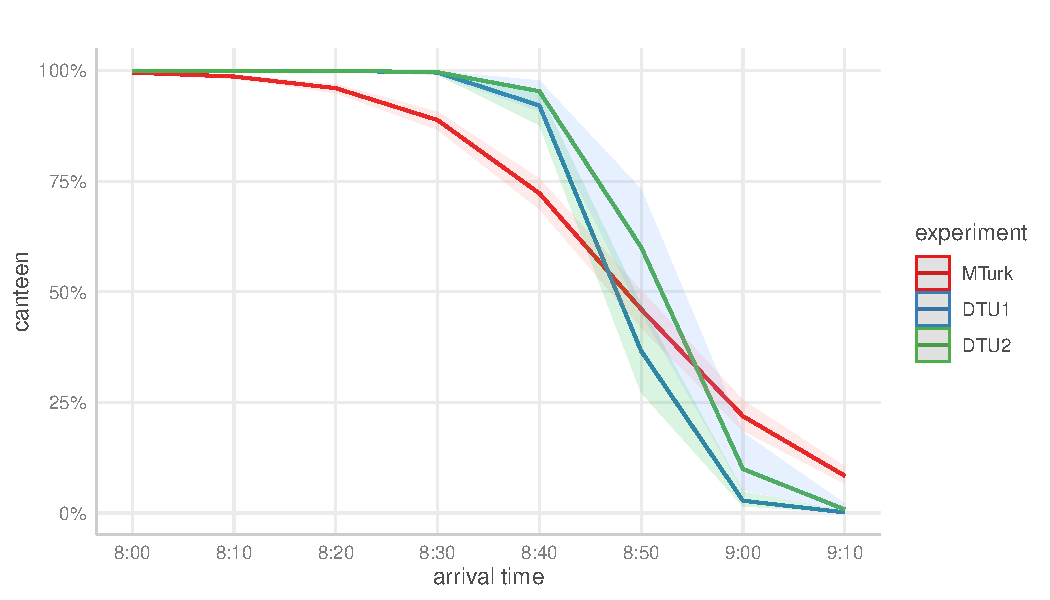
\includegraphics[width=0.8\linewidth]{fig1_regression}
\caption{Percentage of canteen choices as a function of arrival times. The colored lines are logistic regression lines from a mixed-effects model with 95\% confidence intervals shown as translucent bands. Fitted parameters show significant differences in the slope and intercept between MTurk and DTU experiments ($p < .0001$).}
\label{fig:1}
\end{figure}
Using a generalized linear mixed-effects model with the arrival time and the three experimental condition as fixed effects and with player-pairs as random effects, we obtain a logistic regression fit in Fig.~\ref{fig:1}, showing the probability of players choosing the canteen as a function of their arrival time. While DTU students (blue and green) show similar steep profiles with weakly overlapping confidence intervals, MTurk participants in red have a slightly more gradual decline of canteen choices for increasing arrival times. However, the point at which there is a $50\%$ probability of choosing the canteen or the office is close to $8{:}50$ in all three experiments (see further specfications of the regression analysis in Appendix~\ref{appendix:logistic}). Later, in Fig.~\ref{fig:indistinguish}, we make a combined regression analysis of all three experiments in order to understand the overall experimental results in terms of degrees of shared knowledge.

\begin{figure} %[t]
\centering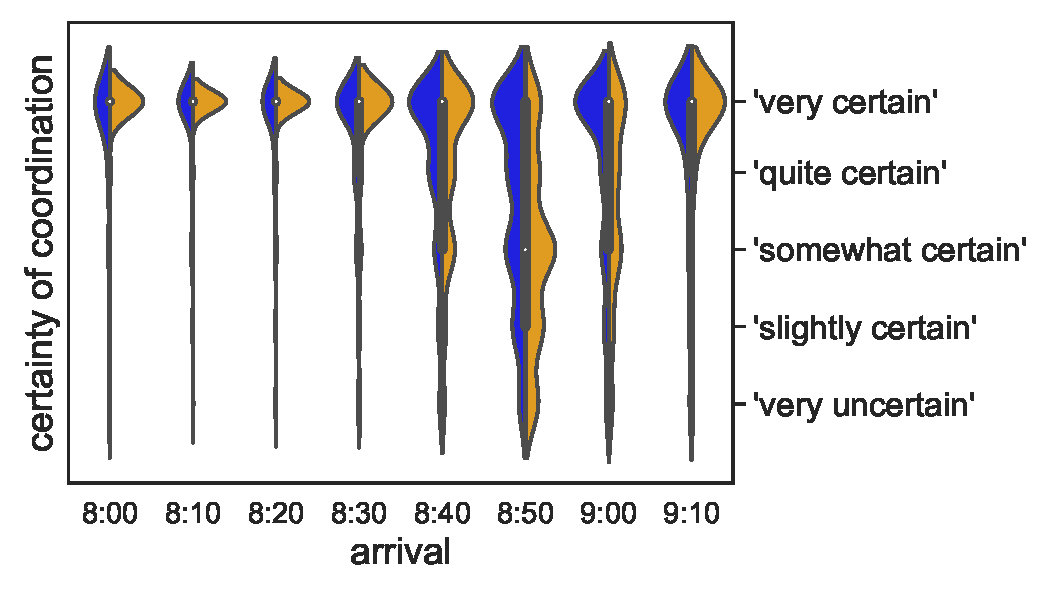
\includegraphics[width=0.8\linewidth]{fig2_certainties}
\caption{Violin plots of certainty estimates. In each round, participants were asked how certain they were of successful coordination with their colleague. Blue areas show the results from MTurk ($n=4260$) and orange areas show the results from DTU1 and DTU2 combined ($n=3172$). We predefined a five point likert scale of certainty estimates as: `very uncertain', `slightly certain, `somewhat certain', `quite certain', and `very certain', and translated them into the numerical values of probability estimates used in the payoff calculations (see Appendix~\ref{appendix:payoffs}). The white dots correspond to the median certainty estimate.}
\label{fig:certain}
\end{figure}

The violin plots in Fig.~\ref{fig:certain} show the distribution of certainty estimates for each arrival time. The DTU experiments are merged and compared with the MTurk experiment, as the differences between the two DTU experiments generally are smaller than their respective difference to the MTurk experiment. This is quantified in Table~\ref{table:1}, as the calculated average penalties per round are a direct consequence of the certainty estimates given by the participants. In general, however, Fig.~\ref{fig:certain} shows that it is exceedingly rare for any of the participants to consider it problematic to go to the canteen when arriving early. Arriving at $8{:}30$ or earlier is deemed sufficiently early to visit the canteen with very high confidence. %, and 
% \tobo{Isn't it more correct to say that that only happens at $8{:}30$ and that $8{:}40$, $8{:}50$ and $9{:}00$ all show some uncertainty? That's how it looks when I look at the violin plots. Only $8{:}30$ and earlier is really robust.} \re{agree. Someone please change to 8:30.} \tsn {Changed the text to 8:30, and adjusted text} 
%arriving at $9{:}00$ or later is deemed office time with high confidence, 
%arriving at $8{:}40$ is deemed either office or canteen with at least being ``somewhat certain''.
%and arriving at $8{:}50$ or $8{:}40$ is deemed either office or canteen with at least being ``somewhat certain''. 
The subtle differences in certainty estimates between MTurk participants and DTU students show that the latter tend to be slightly more certain that their co-players follow a similar strategy (higher certainty estimates for the early and late arrival times), and also that they are more aware of the danger of miscoordination (lower certainty estimates at $8{:}50$ and $9{:}00$). This is in particular the case for the DTU1 experiment that has the steepest profile. Being more certain that your co-players follow a similar strategy probably indicates that you believe such a strategy to be optimal. So, interestingly, the DTU1 participants are both the ones that appear to be most aware of the danger of miscoordination, and at the same time those who most firmly believe a cut-off strategy is optimal, i.e., believing that the risk of miscoordination is unavoidable. The differences between the three experiments are however still relatively minor. In the following we will combine data from all three experiments.

\begin{figure} %[!b]
\centering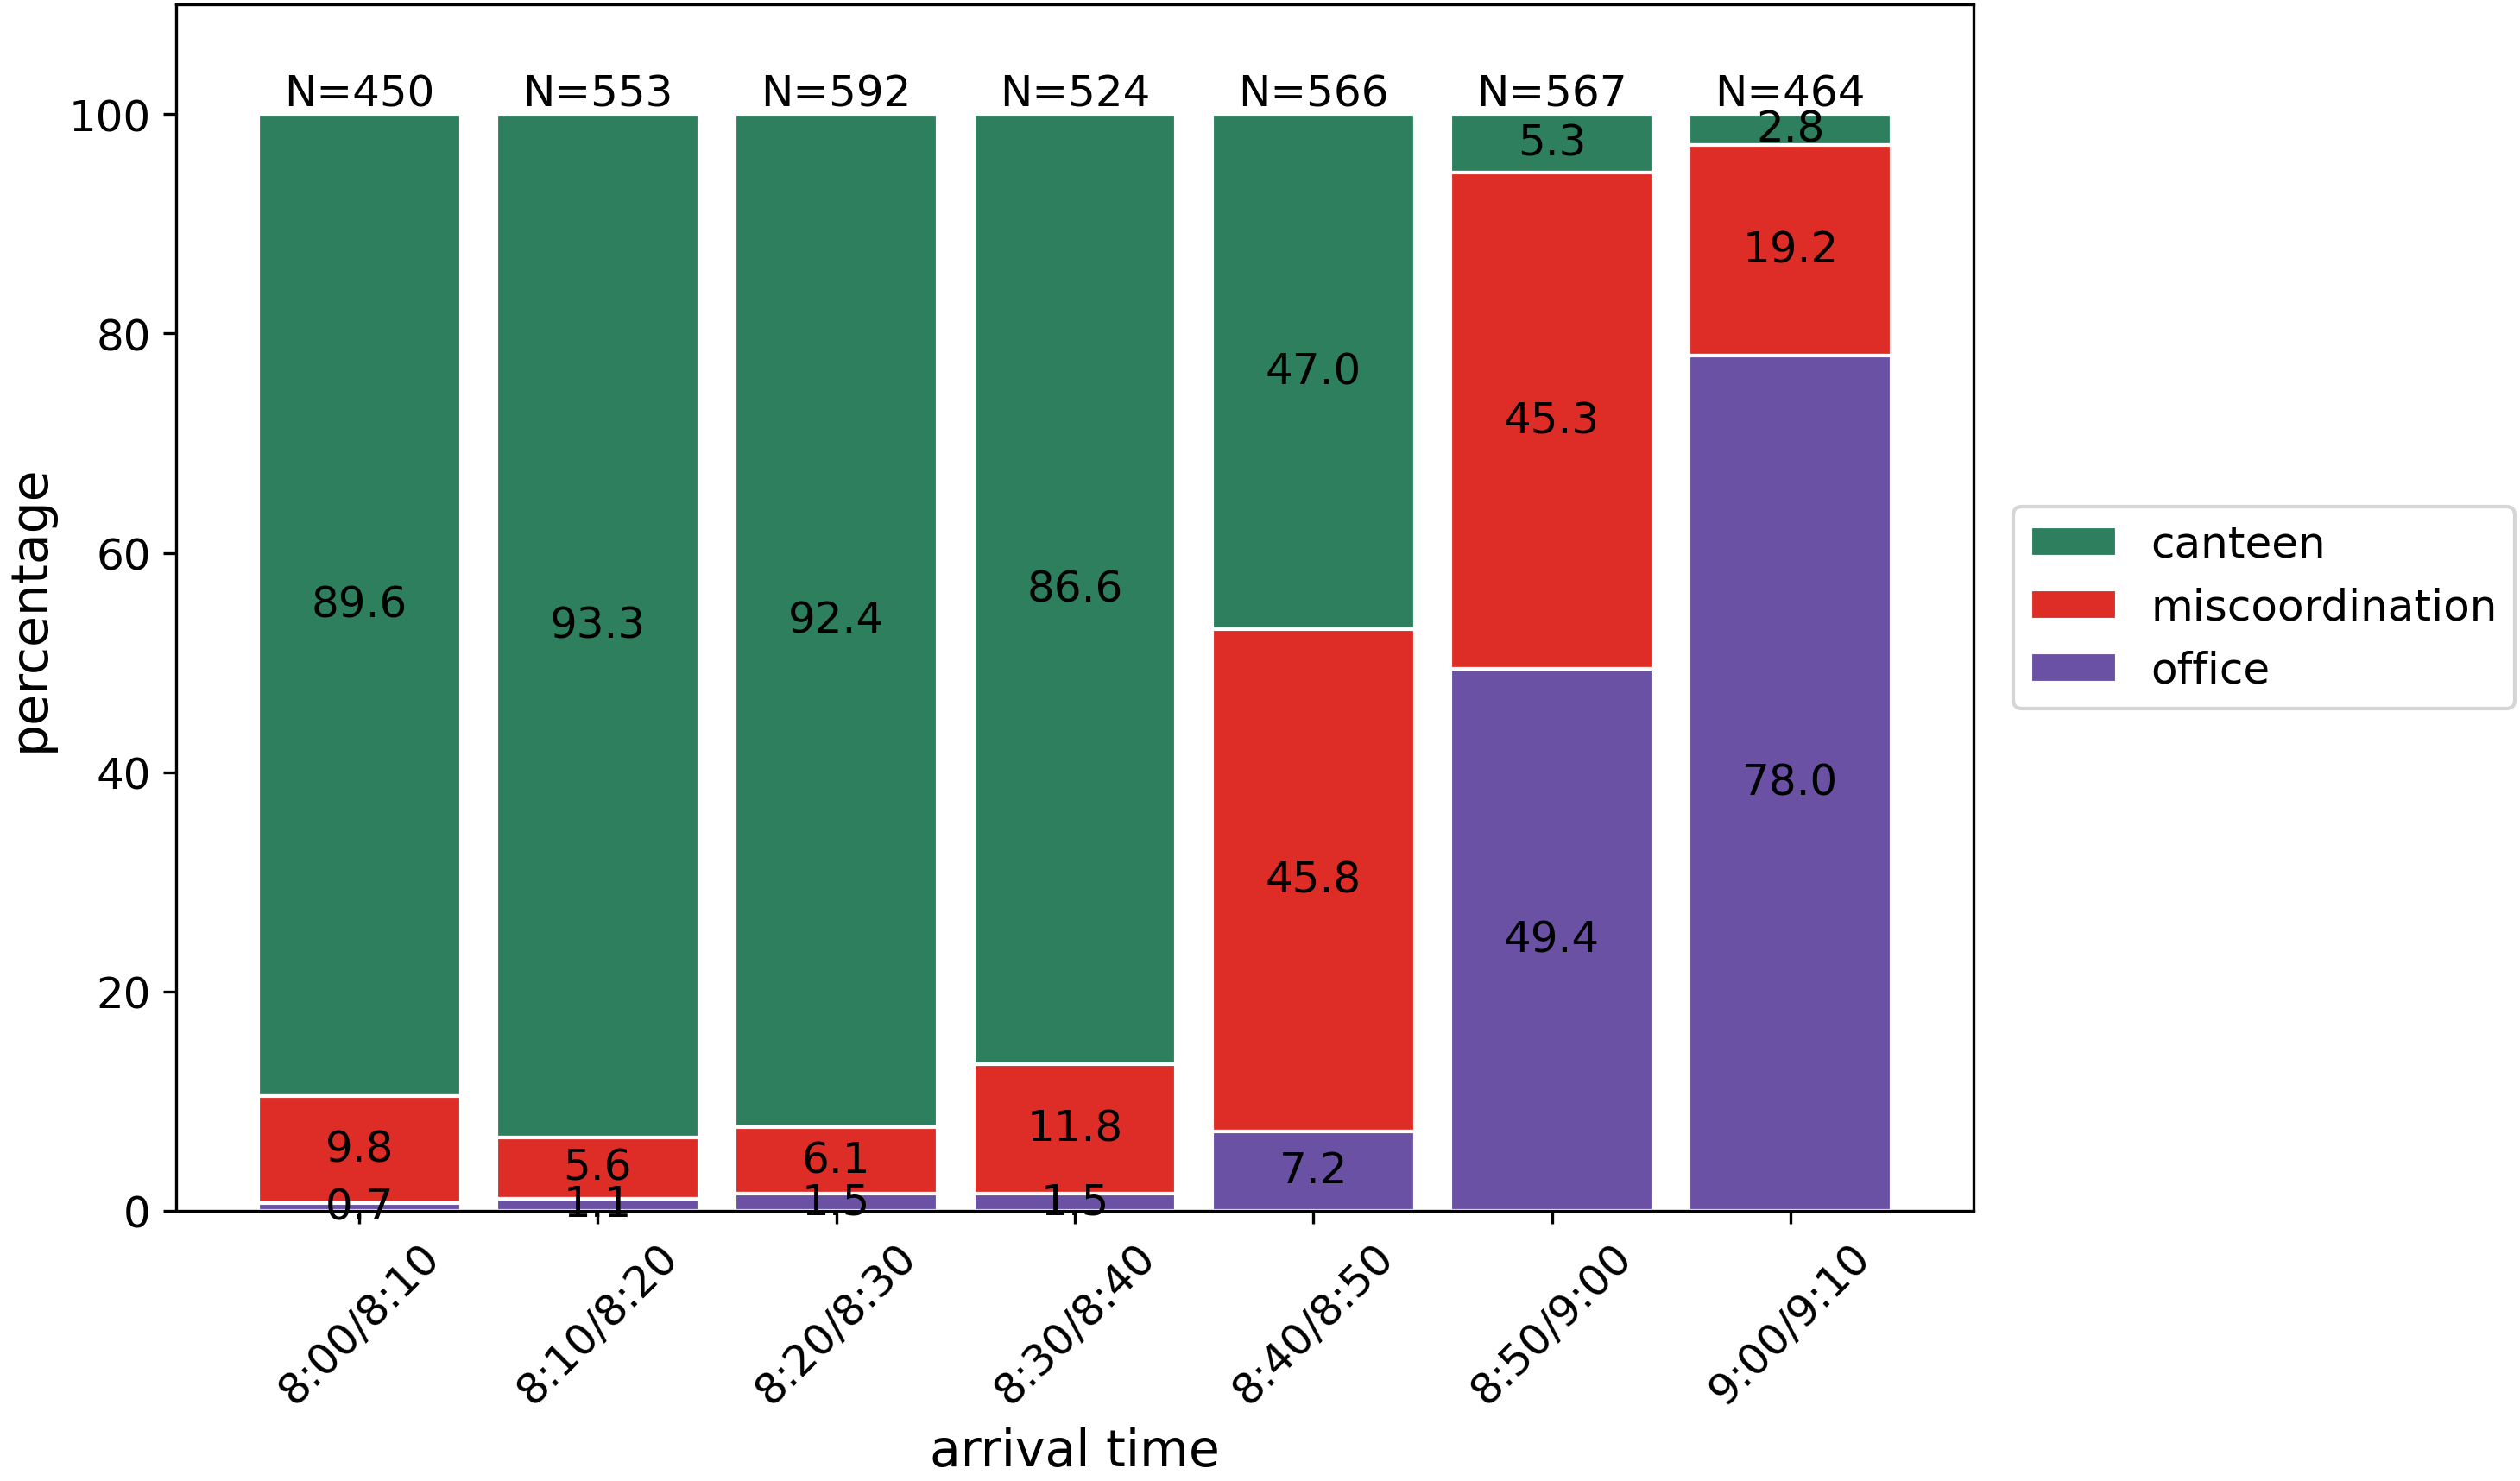
\includegraphics[width=0.8\linewidth]{fig3_miscoordinations}
\caption{Percentage of coordinations and miscoordinations as a function of arrival times. Green means coordinating into the canteen, purple means coordinating into the office, and red means miscoordination. We use the notation 8:00/8:10 to denote the union of the arrival pairs $(8{:}00,8{:}10)$ and $(8{:}10,8{:}00)$, i.e., the arrival time combinations where one of the players arrive at $8{:}00$ and the other at $8{:}10$. Miscoordinations approach $50\%$ at 8:40/8:50 and 8:50/9:00.}
\label{fig:miscoordinations}
\end{figure}

In Fig.~\ref{fig:miscoordinations}, we see the percentage of successful coordinations into the canteen or office (green or purple) together with the number of miscoordinations (red) as a function of all possible arrival time combinations. The figure shows that players are able to coordinate into the canteen more than 86\% of the time if both of them arrive before $8{:}50$. As soon as a pair has a player who arrives at $8{:}50$, however, the result changes drastically. Suddenly almost half of such pairs miscoordinate. As players experience harsh penalties for miscoordinating, one could perhaps expect to see a tendency of choosing office more often when arriving at 8:40 or 8:50 in subsequent rounds. That is, we might expect that players learn and converge to the all-office strategy in order to avoid miscoordination altogether. But this is not what we see.

\begin{figure} % [!t]
\centering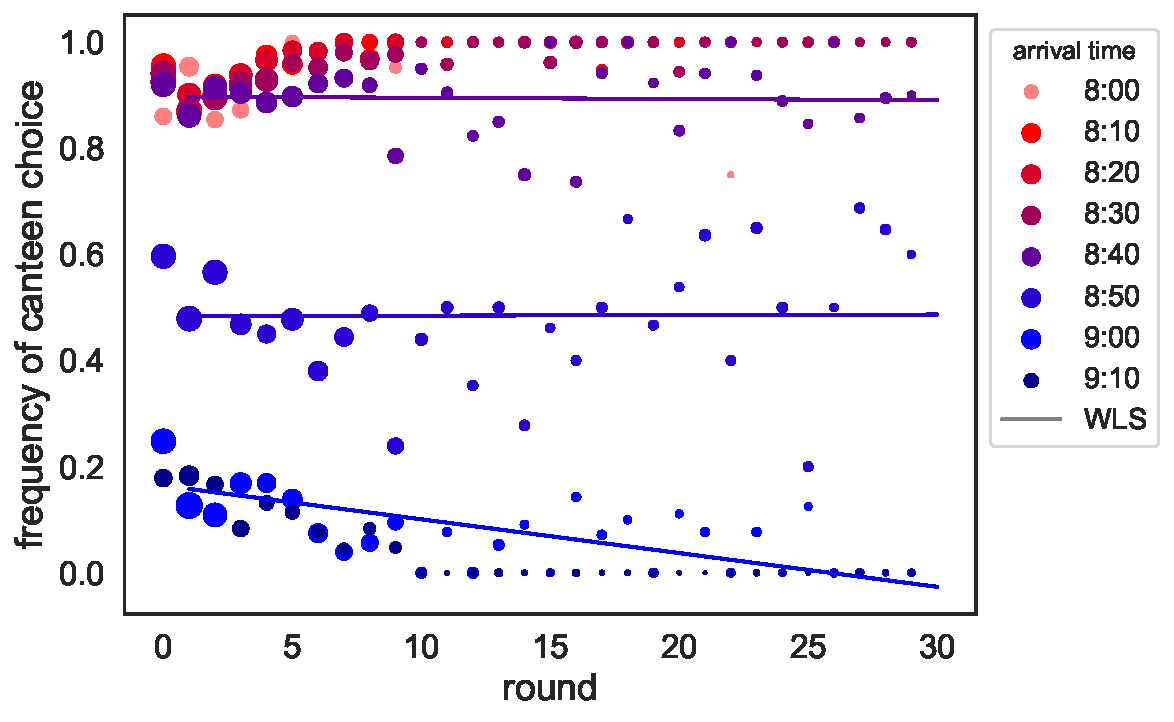
\includegraphics[width=0.8\linewidth]{fig4_timeseries}
\caption{Mean frequencies of canteen choices for all possible arrival times as a function of the number of rounds played. The three fitted straight lines, corresponding to arrival times $8{:}40$, $8{:}50$, and $9{:}00$ respectively, are weighted linear squares (WLS) with the weights chosen to be the square root of the number of data points constituting the mean frequencies for each round, also shown by dot size.}
\label{timeseries}
\end{figure}
Fig.~\ref{timeseries} shows the mean frequency of canteen choices as a function of rounds played for all three experiments. Each color corresponds to a certain arrival time. Clearly, the only arrival times that do not converge towards either the canteen or the office are the arrival times of $8{:}40$ and $8{:}50$, with the former fluctuating around $90\%$ canteen choices and the latter fluctuating around $50\%$ canteen choices. This indicates that there is no behavioral change during the game. Participants arriving at $8{:}40$ or $8{:}50$ do not feel incentivized to change their behavior significantly in subsequent rounds, even though there is a high risk of miscoordination. This is not to say that participants do not learn that canteen choices at $8{:}40$ or $8{:}50$ are dangerous. Partitioning the data from Fig.~\ref{fig:1} into two bins, corresponding to pairs having had no miscoordination and pairs having had one or more miscoordinations (see the supplementary data analysis in the Supplementary Material), shows somewhat decreasing certainty estimates around the critical arrival times. However, this does not affect their actual choices. MTurk participants do choose the canteen a little less often after a miscoordination (see Fig.~6 in the Supplementary Material), but this does not translate into better payoffs as later miscoordinations just move to earlier arrival times. So even though participants learn that their choices are risky, they do not see any way to improve their strategy. Specifically, they never converge to the optimal all-office strategy, and also not to the alternative canteen-before-9 strategy (cf.\ Theorem~\ref{theorem:all-office-or-cut-off} in Appendix~\ref{appendix:formal}). This apparent lack of behavioral change in higher-order social reasoning games is also shown by~\citet{verbrugge2008learning}. 

\add{We also conducted an alternate version of our game based on the Consecutive Numbers Riddle, with players choosing white if they thought both participants had a card lower than 9, and black if either had a card showing a 9 or higher. See Figure \ref{fig:dis} for the results. These show behavior similar to our canteen version, although with more choosing white (similar to canteen) at 8 (similar to 8:50) than in the canteen game. We nevertheless see the same drastic increase in "white" choices in the following numbers. We followed the experiment with interviews with students in groups of 4.  These confirmed both that the players had common knowledge about the rules, as well as the progressive increasing safety of choosing white as the card numbers decreased. Most players believed a cut-off strategy of around 6 or 7 was safe in order to coordinate, although some realized during the interview that such strategy may fail. One was skeptical of any safe strategy existing from the start.}.  \tsn{Skal det beskrives anderledes, så vi beskriver det mindre her?}

\begin{figure} %[t]
\centering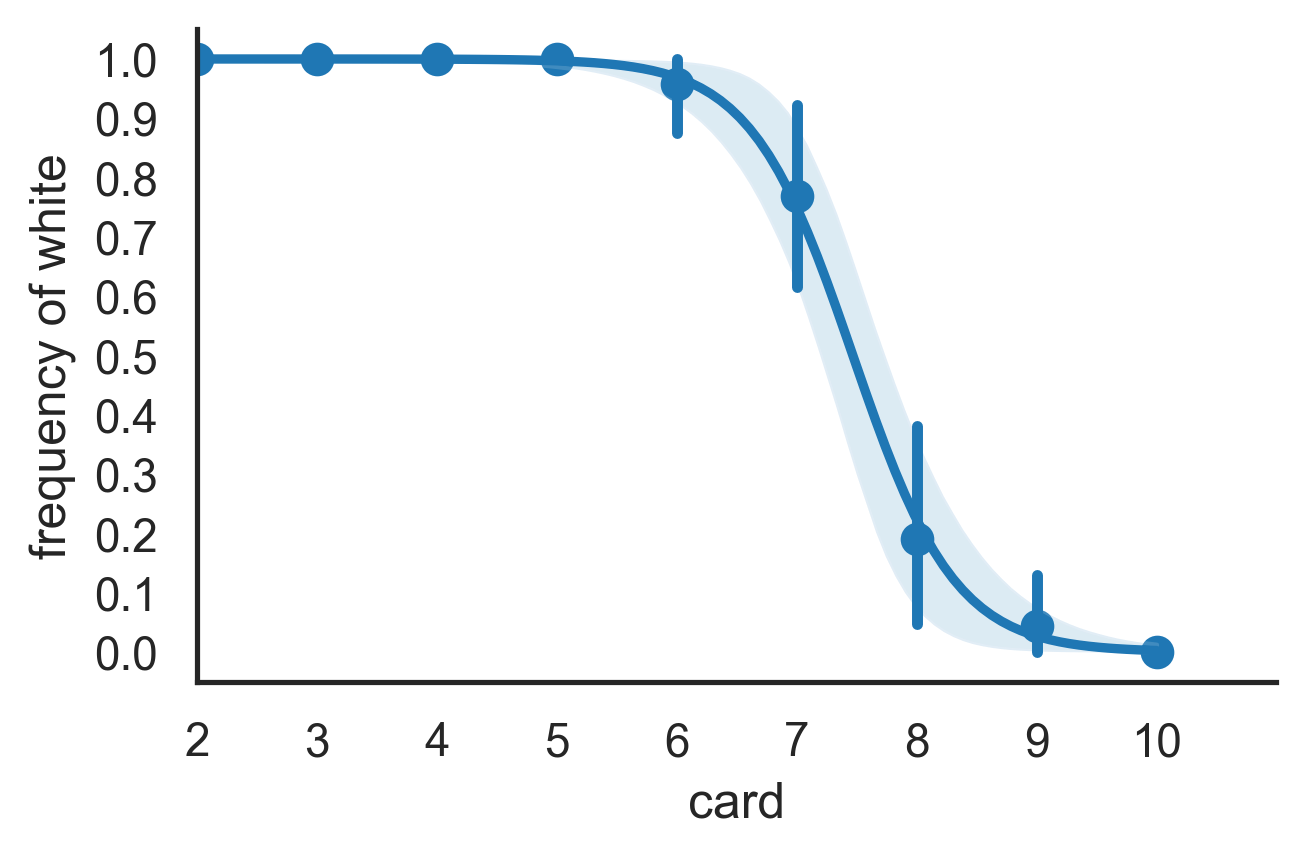
\includegraphics[width=0.6\linewidth]{dis_choices.png}
\caption{XZR.}
\label{fig:dis}
\end{figure}


\section{Discussion}\label{discussion}
Let us try to analyse the experimental results in terms of the depth of knowledge of the participants. The highest payoff is achieved when successfully coordinating into the canteen before 9 am. With the aim of achieving the highest possible payoff, each participant can be expected to consider her own arrival time and try to assess whether there is still time to meet in the canteen. When a participant arrives strictly before 9 am, i.e.\ at $8{:}50$ or earlier, she has private knowledge that she arrives sufficiently early to go to the canteen. If participants only make choices based on their private knowledge, we should then expect participants to always go to the canteen at $8{:}50$. This is not what we see, cf.\ Fig.~\ref{fig:1}. Thus, other considerations in addition to the player's private knowledge must play a role in their decision-making.

When both participants know they arrived before 9 am, they have shared knowledge of having arrived in time for going to the canteen. This happens for any arrival pair $(t_1,t_2)$ with $t_i \leq 8{:}50$, $i=1,2$ (where, again, an arrival pair $(t_1,t_2)$ denotes that player $1$ arrives at time $t_1$ and player $2$ at time $t_2$). Note that for an arrival pair $(8{:}50,8{:}40)$, there is shared knowledge of there being sufficient time to go to the canteen, but only player $2$ knows this fact: Player $2$ knows that also player $1$ must have arrived before 9{:}00, but player $1$ doesn't know this about player $2$. In other words, when a player arrives at $8{:}50$, that player considers it possible that there is shared knowledge of being sufficient time for a cup of coffee in the canteen, but only if arriving at $8{:}40$ or before will that player \emph{know} there to be shared knowledge (to depth 1). When arriving at $8{:}30$ or before, the player additionally knows there to be shared knowledge to depth 2. We illustrate this in Fig.~\ref{fig:indistinguish}. Note that in general, if a player arrives at time $8{:}50-0{:}10n$, $n>0$, then that player knows that there is $n$th-order shared knowledge, but the player doesn't know there to be $(n+1)$st-order shared knowledge. This follows a similar pattern as the mountain trekking example, except here the depth of shared knowledge is determined by how early ahead of 9 am the agents arrive, rather than how many messages have successfully been delivered. No number of messages was sufficient to achieve common knowledge in the mountain trekking example. We similarly get that no arrival time is sufficiently early to establish common knowledge about having time to meet in the canteen. 

\begin{figure} %[t]
\[
  \begin{tikzpicture}[align=left]
   \node[anchor=west] at (-2.6,-2.5) {players' knowledge level of\\ sufficient time for canteen:};
   \node[anchor=west,red] at (-2.6,1) {arrival time player 1:};
   \node[anchor=west,mygreen] at (-2.6,-1) {arrival time player 2:};
   \node[red] (n1820) at (3,1) {8{:}20};
   \node[mygreen] (n2820) at (3,-1) {8{:}20};
    \node[red] (n1830) at (5,1) {8{:}30};
   \node[mygreen] (n2830) at (5,-1) {8{:}30};
   \draw[-] (n1820) to (n2830);
   \draw[-] (n2820) to (n1830);
  \draw[dashed] (4,-3) to (4,1.5);
    \node[red] (n1840) at (7,1) {8{:}40};
   \node[mygreen] (n2840) at (7,-1) {8{:}40};
    \node[red] (n1850) at (9,1) {8{:}50};
   \node[mygreen] (n2850) at (9,-1) {8{:}50};
     \draw[-] (n2840) to (n1850);
   \draw[-] (n1840) to (n2850);
   \draw[-] (n1830) to (n2840);
   \draw[-] (n2830) to (n1840);
  \draw[dashed] (6,1.5) to (6,-3);
  \draw[dashed] (8,1.5) to (8,-3);
     \node[red] (n1900) at (11,1) {9{:}00};
   \node[mygreen] (n2900) at (11,-1) {9{:}00};
    \node[red] (n1910) at (13,1) {9{:}10};
   \node[mygreen] (n2910) at (13,-1) {9{:}10};
     \draw[-] (n2850) to (n1900);
   \draw[-] (n1850) to (n2900);
   \draw[-] (n1900) to (n2910);
   \draw[-] (n2900) to (n1910);
  \draw[dashed] (12,1.5) to (12,-3);
  \draw[dashed] (10,1.5) to (10,-3);
  \node at (13,-2.5) {none};
  \node at (11,-2.5) {none};
  \node at (9,-2.5) {private};
  \node at (7,-2.5) {shared\\ depth 1};
  \node at (5,-2.5) {shared\\ depth 2};
 \node at (3,-2.5) {shared\\ depth 3};
 \node at (7.8,0)
 	{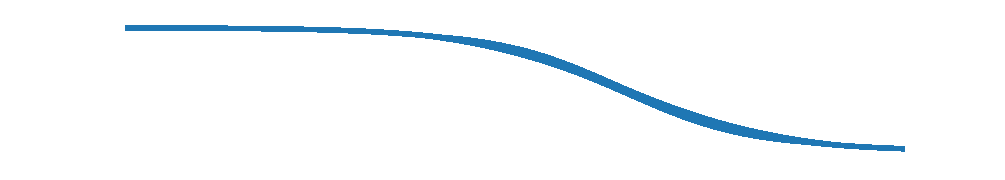
\includegraphics[scale=.75]{fig5_logit_all}};
  \end{tikzpicture}
  \]
  \caption{The solid diagonal lines express indistinguishability for the players, e.g.\ the arrival time $8{:}40$ for player $1$ has a line to both of the arrival times $8{:}30$ and $8{:}50$ for player $2$, since these are the two arrival times for player $2$ that player $1$ will consider possible when herself arriving at $8{:}40$. Below each possible arrival time, we have marked the highest level of knowledge concerning whether there is sufficient time to go to the canteen, e.g.\ when arriving at $8{:}40$ there is shared knowledge to depth 1 of this fact, but not shared knowledge to depth $2$. In blue, a binary logistic regression model was used to predict the probability of a participant going to the canteen (upper limit) or to the office (lower limit) at the shown arrival times. The width of the regression line indicates the 95\% confidence interval using 10.000 bootstrapped resamples of all choices in all three experiments ($n=7432$).
  }\label{fig:indistinguish}
\end{figure}
The participants seem to clearly be able to distinguish between private and shared knowledge, which is supported by their significantly different choices at $8{:}50$ and $8{:}40$ (see again Fig.~\ref{fig:indistinguish}). However, it is less clear whether they are able to robustly distinguish different levels of shared knowledge, and whether they are able to distinguish that from common knowledge. Indeed, most participants relatively robustly choose the canteen at $8{:}40$ and any time before that, despite the difference in depth of shared knowledge in those possible arrival times. The certainty estimates are however slowly decreasing from $8{:}10$ to $8{:}50$ in all three experiments (see Fig.~\ref{fig:certain}), showing that the participants are not completely ignorant to the differences. This could suggest that many participants are aware that it is less safe to go to the canteen based on $n$th-order shared knowledge than $(n+1)$st-order shared knowledge. \tsn{Er det korrekt at det er mindre sikkert ved n end ved n+1? Måske eksperimentelt korrekt, ved ikke om det skal formuleres anderledes?} However, very few seem to draw the conclusion that it is never safe to go to the canteen. Our game theoretic analysis showed that they ought to only choose the canteen when there is common knowledge that it is safe, which in this case actually means never. \tsn{Det afhænger vel af common knowledge om rationel spiller typer, dvs spilteori beskriver at det er optimalt, givet den antagelse, men det er vel ikke nødvendigvis preskriptivt i virkeligheden, hvis vi ikke har den antagelse? Jeg ved ikke om man skal være mere forsigtig her, eller om det er fint/tydeligt at det er i den teoretiske sammenhæng.}

Why do participants not regard earlier office choices as viable options? Why do participants not continue their train of thoughts and deduce that when $8{:}50$ turns out to be unsafe, $8{:}40$ will become unsafe as well, which means that $8{:}30$ will be unsafe also, etc.? One reason may be that the all-office strategy is cognitively difficult to comprehend given humans limited  ability to take the perspective of each other recursively~\footnote{Our experience from playing the Canteen Dilemma with many people and explaining to them its unintuitive result, is that people simply do not accept the argument that there is no time early enough for them to coordinate safely into the canteen. On top of this, when their certainty is challenged by a miscoordination event, they purport that there must be an even earlier arrival time at whice coordinate is certain.} \st{An interesting avenue for future research would be to investigate if there may be any evolutionary or psychological benefits of having such a persistent illusion of common knowledge}. \st{One reason may be that the benefits of an all-office strategy are cognitively unavailable for the participants in the sense that participants have a limited ability to take the perspective of each other recursively [prev. footnote here]}. The computational overload could also be due to the complexity of the game's payoff structure. While this may be a problem, we do not think it has much significance for the following reason. If computational overload was sufficient to distract our participants, we would expect more participants making either random or more uniformly suboptimal choices. While we do see some nonsensically choosing canteen at 9:00, the vast majority choose office at 9:00 and 9:10, and canteen at earlier arrival times, with many still choosing office at 8:50. Besides this, we see participants be much less certain of their canteen choices at 8:50 or 8:40 than at later arrival times. While the game does require quick learning of an unfamiliar payoff structure, we do not believe that it can explain the significant number of office choices at 8:50 and neither the lower certainty estimates. \add{We also note similar results in our followup DIS experiment, see Figure \ref{fig:dis}. This had a much simpler payoff structure of \$1 for coordinating at 9 or 10 (equivalent to office),  \$2 for coordinating at 8 or below (similar to canteen) and losing all their earnings if miscoordinating. }

Another reason besides cognitive difficulties may be that the benefits of an all-office strategy are understood, but participants do not believe that this is common knowledge. \add{That is, they either think their co-player does not realize there is no safe cut-off, or that their co-player thinks this about them, and so on. That is, the game is akin to a Keynesian beauty contest, with an all-office strategy being the optimal equilibrium. In such a case, we would not expect participants to play an all-office strategy, but something else.} One candidate of such a (mixed) strategy may be the following: 1) always go to the canteen before $8{:}50$, 2) always go to the office after $8{:}50$, and 3) do some guesswork at $8{:}50$. The arrival time combinations $8{:}40/8{:}50$ and $8{:}50/9{:}00$ will then coordinate $50\%$ of the time, matching well with what we observe in Fig.~\ref{fig:miscoordinations}. If this is the strategy followed, players should also be aware of the $50\%$ probability of miscoordination at $8{:}50$. In Fig.~\ref{fig:certain}, we indeed see a much lower certainty estimate at those arrival times.

\begin{figure} %[h]
\centering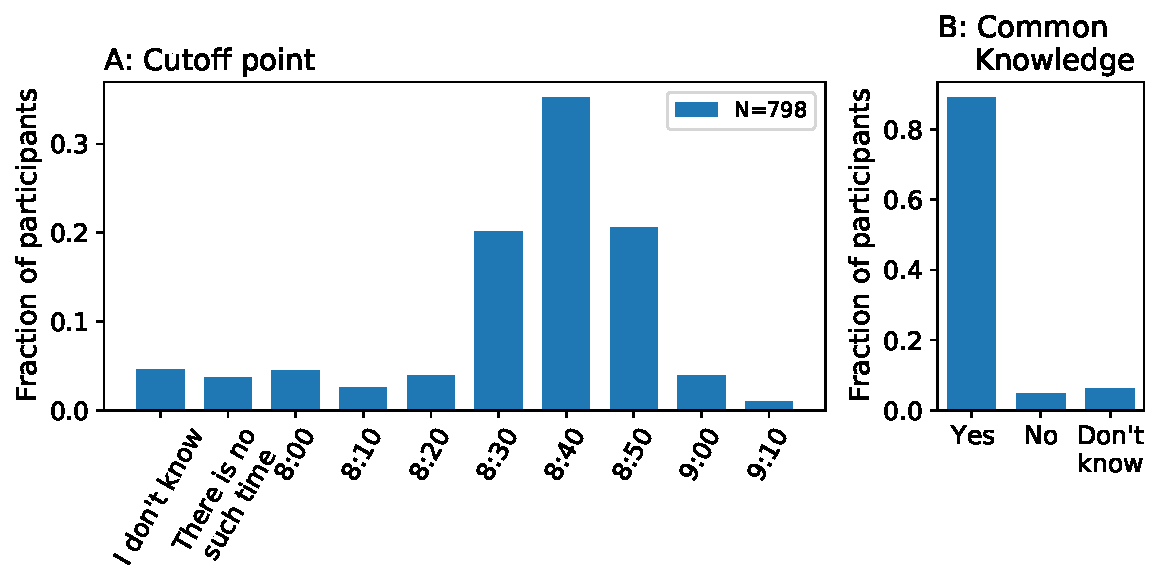
\includegraphics[width=1\linewidth]{fig6_cutoff}
\caption{A) Frequencies of answers to the question: ``Imagine you could have agreed beforehand with your colleague about a point in time where it is safe to go to the canteen. What time would that be?'' Due to the pragmatics of language, we assume that an answer like 8:30 entails the belief that all earlier arrival times would also be deemed safe. B) Frequencies of answers to the question: ``Imagine you arrive at 8:10. Is it common knowledge between you and your colleague that it is safe to go to the canteen, that is, that you both arrived before 9:00?''}
\label{fig:5}
\end{figure}

\add{In other words, players may reason to some degree, but are uncertain about which degree their coplayer reasons.} Probing theses questions further, we asked participants the following post-game question:
\begin{quote}
\indent
``Imagine you could have agreed beforehand with your colleague about a point in time where it is safe to go to the canteen. What time would that be?'' \textit{('I don't know', 'There is no such time', 8:00, 8:10, 8:20, 8:30, 8:40, 8:50, 9:00, 9:10)}
\end{quote}
The results in Fig.~\ref{fig:5}A show that most answers range from 8:30 to 8:50 (approximately $75\%$ of all answers), giving support to the verdict that participants are not able to continue taking the perspective of each other recursively, or at least that they believe that shared knowledge of some modest finite depth is sufficient for the canteen choice to be safe. Rather, they stop after one or two, possibly three, iterations, thus believing that as long as they arrive sufficiently early, they can be sure to coordinate safely in the canteen. Notice that the correct answer ``there is no such time'' is chosen by less than $4\%$ of all participants, close to the margin of random error.

This indicates that participants indeed do believe that there exists a strategy that includes canteen choices without the risk of miscoordination, although in reality they would need common knowledge in order for the canteen choice to be without risk.
% supporting the conjecture stated in the introduction that moderate depths of shared knowledge become effectively indistinguishable from common knowledge.\tobo{Maybe this is one of the places where we could consider to moderate the claim. The question they are asked is not explicitly about common knowledge, and it is not about common knowledge as achieved via public announcements. The question doesn't in itself prove that they can't distinguish shared knowledge of moderate depth from common knowledge. But it shows that they will strategically behave as if they had common knowledge, and will not realise that the unsafety argument can be iterated. So they get "tricked" to believe they can safely coordinate, which means that in some sense their beliefs and actions compare to the common knowledge setting, but I'm not sure we can *strictly* claim the shared knowledge is indistinguishable from common knowledge?}  \tsn {Good point, and I'm not sure, difficult discussion. We want to say that our participants behavior is coextensive with common knowledge behavior. Not sure how to put it. It might be good for various reasons to not focus too much on mental states in general, and look at behavior, but this research field is generally not so behaviorist.} \re{agree as well. We can't really say anything about their understanding of common knowledge from this question. Proposal: remove text starting from ", supporting the conjecture".} \tsn {Support as well.} 
Participants might of course not necessarily have a precise idea of the technical notion of common knowledge and how it differs from $n$th-order shared knowledge, but as discussed in the introduction, there is actually quite a number of studies demonstrating that humans have adapted to recognize common knowledge and making distinct strategic choices depending on whether there is common, shared or private knowledge---at least in cases where the difference between these states of knowledge is relatively clear. In our experiments, we see the player behavior stabilizing already at relatively modest depths of shared knowledge, both in terms of action choices and certainty estimates. And that player behavior does not match what we would expect to see if they only believed to have $n$th-order shared knowledge, but instead matches what we would expect to see if they indeed wrongly inferred common knowledge. 

To specifically address the issue of whether they wrongly infer common knowledge, we asked a final post-game question:

\begin{quote}
\indent
``Imagine you arrive at $8{:}10$ am. Is it common knowledge between you and your colleague that it is safe to go to the canteen, that is, you both arrived before $9{:}00$ am?''. \textit{(`Yes', `No', `Don't know')}
\end{quote}

\noindent
This question inquires about participants' understanding of the term `common knowledge', and how it applies to the given situation. In Fig.~\ref{fig:5}B, the results show that $89\%$ of all participants responded that it was common knowledge that both players arrived before $9{:}00$ when they themselves had arrived at $8{:}10$. The answers may signify that indeed they believe there to be common knowledge in the strict technical (logical) sense. But of course the answers could also pertain to the everyday linguistic usage of the term ’common knowledge’, which is less strict.

\subsection{Ecological Validity} \label{ecovalid}
A relevant discussion relates to how close our experimental setup is to real-world scenarios. We identify a few possible issues here. First, we might ask if participants had a natural preference for canteen outside of the game, which caused them to act sub-optimally in the game. This we find unlikely to be the case. The Canteen Dilemma was evolved from an earlier, purely abstract, version of the game. In this earlier version, the two players each privately received a number in the interval 1-10 and was being told that the other player got a number either one higher or one lower. The players could then choose between two options, A and B. If both chose A and both numbers were strictly below 10, the players would get the highest payoff. If both chose B, they would still get a positive, though much lower, payoff. In all other cases they would lose all their earlier payoffs and the game would end. In this version, the optimal strategy is to always play B (corresponding to the office-only strategy). The only incentive to play A would be to get the higher payoff, but as in the Canteen Dilemma, any strategy which involves A (corresponding to the canteen-choice) will include risk of miscoordination. \st{it is never safe to play A since there will never be common knowledge that both numbers are below 10.} This version of the game \st{The fact that there can never be common knowledge that both numbers are below 10} is known as the consecutive number riddle~\citep{van2015one} or the Conway paradox~\citep{van1980conway}, from where we originally found inspiration for our game. In the original abstract version of the game, we observed the exact same player behavior as in the Canteen Dilemma. Due to the potential opaqueness of the relatively abstract formulation of the original game, we decided for the canteen version, which was believed to be more immediately graspable and potentially more ecologically valid.  \add{We also conducted a followup experiment using this formulation, and found similar results in player behavior. This was corroborated by interviewing the participants after the experiment, which revealed a general belief that some cutoff point or strategy is possible, which involve playing A but does not risk miscoordination. To summarize, we do not believe that players choosing canteen over office reflects a natural propensity towards coffee. }
%We started out with informal testing on people using integer values instead of arrival times, and asking them to coordinate if both got a number below some integer (the consecutive number game \ \citet{van1980conway,van2015one}). We decided against this exactly for reasons of ecological validity, since the abstraction made the game unnecessarily opaque. TODO: Expand this?



Second, we can ask if situations arise in the wild where there is only shared knowledge to some degree but not common knowledge. \st{---and where we would have a tendency to assume common knowledge with potentially large negative consequences}. We will argue that such situations are quite common, \add{especially online.}  \tsn{Vi har måske et problem her, fordi vi beskriver mangel på common knowledge som de tilfælde hvor viden om P ikke er delt af alle (nogle hører ikke efter, eller email ikke når frem). Men det er de simple og lette at forstå tilfælde. Vi vil gerne beskrive den komplekse situation hvor alle ved P, (og måske alle ved at alle ved det etc) men at det stadig ikke er common knowledge. Det er måske mere sandsynligt, hvis vi får en fællesbesked på et medie, som alle læser, men hvor kun nogle svarer. Generelt er problemet nok mere realistisk (indenfor eco. valid.) indenfor online communication, hvilket også er forklaring for hvorfor face-to-face møder er essentielle indenfor vigtige beslutninger} 

\add{Public broadcasting of messages, e.g.\ instructions given in a classroom to a class of pupils or an email sent by the department head to everybody in a university department, will in practice not necessarily lead to common knowledge. Some of the pupils might not be paying attention at the moment, or have misinterpreted the message. Even if they acknowledge it, the same arguement repeats, as the students cannot be certain their acknowledgements were properly received. The error rate for communication in such public broadcasting scenarios is relatively low however. It is worse for online, or written communication. Here it is much less clear if everyone have checked their email, or if the email was correctly delivered. In fact, we know that contrary to face-to-face communication, the messages of emails are rarely read instantly by recipients. So, you cannot cannot be certain everyone have read your email. And likewise, even if everyone sends an acknowledgment email, they cannot be certain that you have read it. }

\st{Public broadcasting of messages, e.g. instructions given in a classroom to a class of pupils or an email sent by the department head to everybody in a university department, will in practice not necessarily lead to common knowledge. Some of the pupils might not be paying attention at the moment, and some of the department employees might not have checked their email, or it might have ended up in their spam filter. Suppose that the message was regarding to all meet at a certain place at a certain time. Can we then be sure that everyone will meet at that place at that time?  Obviously, no.  Then the reply might be that we can just ask everybody to confirm that they received the message, e.g.the school teacher might ask the children to confirm that they heard the message. Well, yes, but then the same argument repeats for the confirmation messages: the recipient of the confirmations might not receive all of them or might briefly not pay attention. }

Now, this generalizes to all social situations and while it does not mean that we do not often obtain common knowledge, it means that we sometimes do not, and end in epistemic situations akin to the canteen dilemma. No amount of confirmations can guarantee common knowledge, and the risk of miscoordination will still be there. However, our hypothesis is that no matter how large the penalty is for miscoordination, when the level of shared knowledge has become sufficiently high, we will act as if common knowledge has already been achieved, it is at least being confirmed in the setting of the canteen dilemma.   . %And probably in most real-life cases the penalty for falsely assuming common knowledge might be somewhat lower than in the canteen dilemma, e.g.\ it might just be that someone doesn't show up for the event that the original message concerned. 

\add{Third, we may ask whether people reason and behave in real world scenarios similar to how they do in our game, even if they seem structurally similar. This requires more antropological research on real life scenarios to establish. In any case,  we have not found that people can distinguish between all levels of shared knowledge and common knowledge at least within the experimental setting, which is a refinement of \cite{thomas2014psychology}.  }

We also note that in most everyday situations, the penalty for confusing shared knowledge with common knowledge is probably much lower than in our game. If it is for instance a group of pupils who are asked to meet at a certain time and place to get on the bus home from a school trip, confusing shared knowledge with common knowledge is not likely to be a big problem. It just means that the children will meet at the designated time and place despite not having common knowledge that all other children will also be there. In this case, the confusion of shared knowledge with common knowledge might even be helpful, since it allows coordination despite the lack of common knowledge. But this only happens because there is no large penalty if coordination fails. Even if one child eventually doesn't show up, it is probably better for all the other children to arrive anyway rather than not going due to the risk of someone else not showing up. In certain cases, it could however be different. \tsn{Måske skal vi ændre/slette eks. ovenfor?} \add{ Say you write an email to people saying you will buy an expensive plane ticket for them for a trip, unless they cannot go. If a person does not answer, you cannot be certain if they in fact wont show up, but just have not read your email, resulting in you buying a ticket for nothing. So, you decide to write that you only buy tickets for those who answer your email. Even if they acknowledge your email, and you read it, they might still not be certain you have read the email in time, so they buy a plane-ticket for themselves, leaving you both buying tickets. And even if you acknowledge their acknowledgement, you cannot be certain they read it, in which case you know they will buy a plane ticket. This may you to not buy a ticket for them, but where they don't do so either, since they in fact did read your acknowledgment. We may intuivetively avoid such cases where miscoordination is costly, either by making rules such that no coordination is necessary (everyone fends for themselves) or by making agreements face-to-face.  Our experiments show however that when we are in such situations, we do not seem to understand the impossibility of coordination, even after multiple miscoordinations. This is not to say that we should not try to coordinate, but that we should consider the risks of miscoordination if we coordinate in writing } \tsn{Det er måske dumt at have noget normativt med her? Det er et forsøg på at bygge ovenpå eco. validity pointen}
%The problem of these scenarios is two fold. First, such scenarios are difficult to grasp, as our experiments have shown, making it harder to see the possibility of miscordination. Second, our intuition concerning such scenarios are likely determined by the possibility of faulty communication and the consequences of miscoordination. That is, we might not grasp the chance of miscoordination if its consequences are sufficiently small.

In general, if a group tries to coordinate a public demonstration, a dangerous emergency rescue or coordinate to all write letters of complaint, they might suffer a high penalty if a sufficiently high number of group members end up not participating. In this case, confusing shared knowledge with common knowledge can be critical, and it can be critical to be in a situation where common knowledge cannot be achieved (e.g.\ if trying to coordinate via posts on social media or trying to shout through the walls of a burning building). 
% go home from a school trip 
%For instance, in the example above it might just be that someone doesn't show up at the agreed place and time, and though this could lead to a high penalty for those who don't show up, it might not lead to a high penalty for everybody involved in the coordination effort. However, there \emph{could} be such a high joint penalty, e.g.\ if the class is supposed to meet for the bus to get home from a trip to a museum, and then...
%this might not lead to a high penalty for everybody involved in the coordination task. 


Still, probably in most real-world scenarios, the penalty for miscoordination is lower than in our canteen dilemma. However, if that is indeed the case, then we should expect humans to pay \emph{more} attention to the potential confusion of shared knowledge for common knowledge in the game than in the wild.  In other words, if participants do not pay attention to it in our game, we should not expect them to be more aware of it in the wild.



We might have evolved to do our best to avoid such situations, due to the complexity involved. This might explain why we do not identify it everywhere in our daily life. But it is unlikely that we can categorically deny that such situations arise. \st{and when they do, some might implicitly assume common knowledge to be present, while others, on a lower order of shared knowledge might not.} This results in miscoordination which people cannot predict, and possibly not even post-hoc understand. 


\section{Conclusion} \label{S:conclusion}
We have devised a new coordination game, the Canteen Dilemma, to investigate human higher-order social reasoning. Our experimental results show that high levels of recursive perspective-taking are cognitively unavailable to the vast majority of players of the game. We see a significant amount of miscoordination, which seems to occur due to a ``curse of shared knowledge'': an illusion of common knowledge in situations where there is only shared knowledge to some limited depth. For some people it may not seem surprising that people behave as if they have common knowledge in shared knowledge situations and that they are not able to improve upon their behavior despite huge penalties. However, the existing research literature suggests that it \emph{is} surprising. Findings by~\cite{rubinstein1989electronic, lee2010rationales, thomas2014psychology, thomas2016recursive, thomas2018common, de2019common, de2019maimonides} suggest that people make strategically different choices depending on whether they have shared or common knowledge. A crucial difference between their and our results is the difference in the experimental design: While previous studies rely on a detailed explanation of the level of common or shared knowlege among participants in their group, our study does not make any such explications. Instead, the level of knowledge in our design needs to be \emph{deduced} by the participants. This, we believe, is an ecologically more valid approach, because people in real life situations rarely are given explicit explanations about what is known by whom. Our methodology of using arrival times thus opens up the possibility to investigate more realistically the vast space of shared knowledge dynamics among coordinating humans. One might have predicted that the added complexity of asking participants to be able to deduce the relevant levels of knowledge would make them conclude less, that is, assume a lower level of shared knowledge than is actually there. This is because bounded reasoning capabilities most often lead agents to conclude less than what a resource-unbounded agent would be able to conclude~\citep{fagin1995reasoning, halpern2011dealing}. However, surprisingly, we observe the opposite: agents seem to infer, or act as if they had, common knowledge when it is not there. 
%make you able to conclude less than what logically follows from you knowledge).  

We suggest that our game design constitutes a methodological advancement in the field of cognitive science due to its ability to replace complicated experimental explications of who knows what, or long stories about unreliable message passings, with asynchronous arrival times. It reduces experimental error and increases paradigmatic flexibility. Our contribution also goes well beyond a pure methodological advance. Our main theoretical contribution is that non-explicated higher-order shared knowledge is wrongly treated as common knowledge in realistic settings where humans can't (or won't) communicate freely, even when they could deduce that common knowledge is unattainable. This means, informally, that bottom-up sensory stimuli ("the time is before 9 am") \emph{wins the perception battle} over top-down conceptual knowledge ("she could think that I think that she thinks ..."). And this is the case despite repeated error signals. We are confident that this is of theoretical importance for various subfields within the cognitive sciences such as predictive processing~\citep{hinton2007learning, palmer2015felt}, stigmeric coordination~\citep{heylighen2016stigmergyI, heylighen2016stigmergyII}, multi-robot and human-robot interaction~\citep{devin2016implemented,lemaignan2017artificial,nebel2019implicitly,dissing2020implementing,bolander2021del}, as well as for Theory of Mind~\footnote{It should be noted that recursive games do exist in the ToM literature, see for instance~\cite{hedden2002you, flobbe2008children, curry2012putting}. Our purpose, however, is not to determine whether players can distinguish $n$th-order and $(n+1)$st-order shared knowledge, but whether players can in general distinguish shared knowledge (of some order) from common knowledge.}.

\st{We believe that our results may also be of practical interest for legislative efforts trying to create social rules of conduct in situations where coordination without explicit communication is common. By way of example, we may mention recent changes in global legislations on sexual assault: within the last 20 years, more than 30 countries globally have shifted or are in the process of shifting from a coercion-based model, which requires that for a sexual act to be considered rape there needs to be proof of coercion, to a consent-based model. The latter stipulates that sex without mutual consent is to be considered rape. The main reason for this change is that sexual assault often occurs in situations where friends or partners miscoordinate their signals and become unable and/or unwilling to change their behavior %~\citep{mcgregor2017rape, amnesty2018yes, koljonen2019how, wikipedia2021sexual}.  
In other words, sexual consent law frequently deals with ambiguous coordination problems where private or shared knowledge has been erroneously interpreted as common knowledge. Consider the following real world scenario: instead of Agnes and Bertram meeting at the top of a mountain or for a cup of coffee in the canteen, we look at them trying to to interpret certain behavioral signals of each other as either romantic or not ("she/he makes a certain comment", "he/she touches you", etc..), and decide whether they want to make a sexual advance or not. The issue is that it might not be enough that the other is interested, certain actions requires consent as well to be permissible, like most touching of a sexual kind. The question then becomes: at which point may a direct sexual advance be permissible, if ever? If only one of them is interested, it is clearly wrong to make a move. If both are interested, but don't know whether the other one is as well, they still ought to refrain from action, as they can't be certain that the other one is interested. Suppose now that it is shared knowledge that both are interested. Then they both individually know that the interest is mutual. However, if it is only first-order shared knowledge, Agnes doesn't know that Bertram knows that the interest is mutual. Hence, if Bertram makes a sexual advance, Agnes considers it possible that he is making the advance without knowing that the interest is mutual. Hence, Agnes considers it possible that he is making an advance in one of the situations where he clearly shouldn't, which Agnes might very reasonably see as off-putting or at least as raising a red flag. The conclusion is that even first-order shared knowledge is not in general sufficient for it to be appropriate and safe to make a sexual advance. The argument may be repeated to show that even second-order shared knowledge is insufficient: If it is inappropriate for Bertram to make an advance based on first-order shared knowledge, it will likewise be inappropriate to make an advance based on second-order shared knowledge, as Agnes will then still consider it possible that Bertram is making an advance based on first-order shared knowledge only.   The point, of course, is that this can be generalized in the same way as in our game. As long as there is not established common knowledge about consent, any behavior that relies on a cut-off point between an action being permissible at one epistemic level but not permissible at another, will necessarily lead to miscoordination, which in the romantic case may amount to anything from awkwardness to harassment. Thus, it follows that we must either accept the risk of miscoordination, or stick to inaction until we have achieved common knowledge about mutual consent. Common knowledge about mutual consent can only be achieved via explicit agreement beforehand. Traditionally, sexual advances have most likely been made on the basis of less reliable romantic signals that only would guarantee shared knowledge (or shared belief) to a certain depth.}

So the wider implications of our findings are these: If we do not take seriously the fact that we often are unable to properly distinguish between common knowledge and shared knowledge, we cannot hope to mitigate the harmful effects arising from it. Players in the Canteen Dilemma might not appreciate the importance of a public announcement that they both arrived before 9:00am \add{ if they both know this, arriving at 8:30 and 8:40}. But they may run into miscoordination without it. \add{As epistemic logic teaches us, public information about something everyone knows can still provide crucial knowledge to us.} \st{The same applies for the parties in a potential romance: they may not think highly of explicit announcements and mutual agreements, but risk doing irreparable harm without.} Our results therefore show the importance of emphasizing open, honest and reliable communication, even when not intuitively necessary, in situations where it matters. 


%An obvious question is how often this illusion of common knowledge occurs in real life. For instance, in the real-world version of the Canteen Dilemma scenario, the two colleagues would be likely to simply coordinate their actions via cell phone (``I'll arrive at 8:50 today. Are you up for a cup of coffee in the canteen?''). This suggests that the advent of modern technology could have made the information asymmetry inherent in shared knowledge situations less widespread. However, modern technology has also given us the Internet and social media, where the flow of information is much more complex, creating more intricate cases of information asymmetry than ever before. 

%That humans tend to confuse shared and common knowledge could possibly be due to a limited evolutionary importance of being able to make the distinction. It could also be due to the distinction requiring too many cognitive ressources. Or it could be that the confusion actually leads to evolutionary benefits in terms of higher degrees of cooperation in most practically occurring settings. What exactly has lead to the confusion, and to what degree it has any practical importance today, we leave as open problems.


%--> paragraph on limitations. 
%--> paragraph on future work

\clearpage


\if\cogsci 1
\bibliographystyle{apacite} %model1-num-names}
\bibliography{cd}
\fi


\appendix

%\section{Materials and Methods}\label{sect:materials_methods}
% \tobo{Why is the section not called Material and Methods?} \tsn{As far as I can tell: We should change "Methods" here and above to "Material and Methods". We refer to both, and as far as I can see, the references are to material in the section below. UPDATE: Changed all instances of "Methods" to "Material and Methods"}

 %\small

\section{Experimental design and data collection} A large total sample size of $N=870$ was chosen to get robust conclusions from the statistical analysis while giving room for high variability in behavior. In fact, we thought that there would be a minority of pairs who would meet in the office all the time. This turned out not to be the case. Experiments on Amazon Mechanical Turk had a total of 714 participants (including dropouts, see Supplementary Material), while the two classroom experiments at the Technical University of Denmark (DTU1 and DTU2) had a total of 106 and 50 participants, respectively\footnote{Complete anonymized data files and all code can be downloaded from \url{https://github.com/gavstrik/Paper_canteen_dilemma}.}

The average payout to MTurk workers was \$4.17 (including a general participation fee of \$2). After accepting our task and providing informed consent, participants from MTurk were put in a ’waiting room’ until they were paired up with another participant. After an instructions page, detailing the rules of the game, participants were given an arrival time $t \in \{8{:}00, 8{:}10, 8{:}20, 8{:}30, 8{:}40, 8{:}50, 9{:}00,9{:}10\}$ and asked to make a decision between between going to the canteen or to the office. Next, participants were asked to estimate how certain they were that their `colleague' made the same choice as them, ranging from `very uncertain' over `slightly certain', `somewhat certain' and `quite certain' to `very certain', which were translated  into numerical values, $e_i$, used in the payoff calculations (see below). A results page was shown between each round, showing the results of the previous rounds, including arrival times for both players, their choices, their own certainty estimates and resulting payoffs. After 30 seconds, the game would automatically proceed to the next round. After the last round, we asked all participants a few final questions about their strategy and their understanding of the game. The experiments were implemented using oTree 2.1.35~\citep{ChenSchongerWickens16}.

The two classroom experiments DTU1 and DTU2 differed from the MTurk experiment in a few aspects: 1) the maximum number of rounds played was increased from 10 to 30; 2) the initial bonus given each participant was increased accordingly from \$10 to \$30; 3) three additional questions were asked in order to elicit more explicitly some of the implicit assumptions and explicit behaviours by the students; 4) participants were told that they would not receive any monetary rewards, but that they should try to do their best. DTU1 received prizes. Screenshots, additional questions, experimental settings, and a detailed walk-through can be found in the Supplementary Material.

\subsection{Mixed effect logistic regression} \label{appendix:logistic} 
The experimental results were analyzed using a generalized mixed-effects logistic regression model in R (\emph{glmer}), with the arrival time $t$ and experimental condition $exp$ (MTurk, DTU1, DTU2) as fixed effects including interactions and random effects for each pair of players, because we expect pairs to behave differently, depending on which levels of shared knowledge they individually take into account in their reasoning and collectively try to agree upon. Exploratory analysis including the round number as additional fixed effect did not show any significant contributions, meaning that players did not significantly change their strategy during the game. %The model was specified as $\mu_i = \alpha _{i} + \beta _{i}t + W_{ij}$, with $\mu_i$ being the log-odds $\mu_i= \log (p_i/(1-p_i))$ and $W_{ij} is the pair-specific random effect, i.e., it's the deviation of the j-th pairs’s score from the average for the i-th experiment. $i=1,2,3$ denoting the MTurk, DTU1 and DTU2 experiments, respectively, allowing for differing slopes and intercepts. 
Results from the fitted model are shown in Fig.~\ref{fig:1}. The steepest slope occurs at $p(t) = 1/2 = -\alpha/\beta$, which for the MTurk and DTU1 experiments is $t=8{:}48$ and for DTU2 is $t=8{:}52$. The regression line in Fig.~\ref{fig:indistinguish} is obtained by combining observations from all three experiments and using a simple logistic regression model without random effects. The high number of observations imply small confidence bands. Hence, conclusions from the models can be viewed as robust. Code and data are available on github.


\section{Payoffs and Penalties} \label{appendix:payoffs}
 All MTurk players finishing the game were paid a participation fee of \$2. In addition, a bonus could be earned if players did well. Before the game started, the bonus was set to \$10 for all participants. After each round, the bonus was reduced by a personal penalty, depending on the two players' choices. Penalties are calculated using a logarithmic scoring rule and by ordering them to be minimized by successful coordinations into the canteen. Penalties are maximized by any type of miscoordination or forbidden choice (i.e.\ going to the canteen at 9 am or later). Office coordinations are designed to have larger penalties than canteen coordinations, but smaller penalties than miscoordinations in order to make sure that coordination remains the main objective of the game. Penalties are defined as negative utility values in the following way. First, we define the chosen action $a_i$ by player $i$, $i=1,2$, to take binary values encoding the canteen option ($a_i=0$) and the office option ($a_i=1$), and define their respective certainty estimates $e_i \in \{0.5, 0.625, 0.75, 0.875, 0.99\}$. We can then express the utility $u$ received by player $1$ as $u(e_1, a_1, a_2) = (1-|a_1-a_2| + a_1a_2)ln(e_1) + 2|a_1-a_2|ln(1-e_1)$, and symmetric for player 2. If any of the players choose the canteen at 9 am or after, the utility becomes $u(e_1,a_1,a_2) = 2ln(1-e_1)$ for player 1 (and symmetric for player 2), corresponding to a miscoordination. As an example, imagine player 1 arrives at $8{:}40$ and choses the canteen, $a_1=0$. She estimates the probability that her colleague also will to go to the canteen to ``somewhat certain'', $e_1=0.75$. If her colleague indeed chooses the canteen, $a_2=0$, her utility will be $u(e_1,a_1,a_2) = ln(e_1) = -0.29$, but if her prediction proves false and her colleague chooses the office instead, her utility will be $u(e_1,a_1,a_2) = 2ln(1-e_1)=-2.77$. If she goes to the office just like her colleague, her utility is $u(e_1,a_1,a_2) = 2ln(e_1)=-0.58$. It should be noted that the logarithmic scoring rule used here is strictly proper. Therefore it is not surprising that we find a good match between estimates and actual choices at arrival times different from those that are prone to miscoordinations, as seen in Fig.~\ref{fig:certain}, indicating that loss minimization remained a central concern and that participants made their choices and estimates as honestly as possible \citep{good1992rational, seidenfeld1985calibration, palfrey2009eliciting}.

\section{Formal Analysis} \label{appendix:formal}
We now give a detailed formal analysis of the game. We want to keep things as general as possible, so we don't assume a particular payoff structure, but any payoff structure satisfying certain constraints, and we want to consider arbitrary strategies, also mixed ones. This makes the analysis a bit non-trivial, although the underlying intuitions are rather straightforward. We of course haven't expected our human subjects to have made a deep analysis corresponding to the one below before starting to play the game. That should also not be necessary: The crucial aspect is to realize that there is no time point at which it is safe to go to the canteen (and hence avoid the high penalty), and this only requires to reason that 8{:}50 is not safe, and that then also 8{:}40 is not safe, and that then also... etc. What we do below is just to verify in a generalised setting that this reasoning is indeed formally correct and game theoretically valid and acting according to it leads to the highest expected payoff.  

The game can be represented as a game with three players, \emph{nature}, \emph{player 1} and \emph{player 2}. Nature is the player that initially decides the arrival times of player 1 and 2. Then player 1 and 2 are each informed of their own arrival time, and each have to choose among two actions: $o$ for going to the office and $c$ for going to the canteen. Based on the choice of actions by all three agents, player 1 and 2 receive a payoff, and they always receive the same payoff (we are disregarding the certainty estimates for now). The action choice of nature can be represented as an \emph{arrival pair} ${\bf t} = (t_1,t_2)$ consisting of the arrival time $t_1$ for player 1 and $t_2$ for player 2. Any arrival pair $\bf t$ has to satisfy that  $| t_1 - t_2 | = 10$ minutes (we will suppress mentioning the unit, minutes, in the following). In our specific version of the game, we additionally have the restriction that $8{:}10 \leq t_i \leq 9{:}10$ for $i = 1,2$. The analysis of optimal strategies however doesn't depend on the exact arrival times available, so we will make things a bit more general and only assume that there is an earliest arrival time $\tmin$ and a latest arrival time $\tmax$, and that $\tmin \leq 8{:}50$ and $\tmax \geq 9{:}00$. Since we are counting in 10s of minutes, by slight abuse of language we will call an arrival time \emph{even} if it is of the form $9{:}00+20x$ for some integer $x$, and an arrival time \emph{odd} if it is of the form $9{:}00+10+20x$. The game then naturally splits into two disjoint subgames. In one of these subgames, player 1 always arrives at an odd time, and player 2 at an even time. 
%arrives at a time $\tmin+20x$ for some $x \geq 0$ and player 2 arrives at a time $\tmin+20x+10y$ for some $y \in \{-1,1\}$. 
 In the other subgame, the arrival time of the two players are reversed. The two subgames are disjoint in the sense that it is always common knowledge among the players which of the two arrived at an even time. We can hence restrict focus to one of the two subgames. We will pick the subgame where player 1 arrives at an odd time. To simplify further, we can without loss of generality assume that both $\tmin$ and $\tmax$ are also odd times. All reasoning performed in the following generalises immediately to the other subgame and to other values of $\tmin$ and $\tmax$. 
 
We let $T$ denote the set of arrival times and $\bf T$ the set of arrival pairs.  
The game starts by nature choosing an element $\mathbf{t} \in \bf T$. Nature is not a strategic player, so we assume that $\bf t$ is chosen uniformly at random, which is exactly how $\bf t$ is chosen in our experiments. The participants do not know that the arrival times are chosen uniformly at random, as this is left implicit in the description of the game. The following analysis of optimal strategies in the game could potentially change if arrival times were chosen according to a highly skewed probability distribution.

When nature has chosen its action ${\bf t} \in \bf T$ and player 1 and 2 have chosen their actions $a_1$ and $a_2$, player 1 and 2 receive their payoff, which we denote $u_\mathbf{t}(a_1,a_2)$ (the utility resulting from player 1 choosing $a_1$ and player 2 choosing $a_2$ given that nature played $\bf t$). We don't need to make any assumptions regarding the exact utility values (payoff values), except that successful coordination into the canteen before $9{:}00$, denoted $u_\mathit{c}$, is always better than successful coordination into the offices, denoted $u_\mathit{o}$, which again is always better than being miscoordinated, denoted $u_\mathit{m}$. Hence we suppose given fixed utility values $u_\mathit{c} > u_\mathit{o} > u_\mathit{m}$ such that for all ${\bf t} = (t_1,t_2) \in {\bf T}$,  $u_{\bf t}(o,o) = u_\mathit{o}$, $u_{\bf t}(o,c) = u_{\bf t}(c,o) = u_\mathit{m}$ and 
\[
u_{\bf t}(c,c) = 
\begin{cases}
   u_\mathit{c} &\text{if $t_1,t_2 < 9{:}00$} \\
   u_\mathit{m} &\text{otherwise}
\end{cases}
\]
 % such that 
%Hence, we put the following constraints on the utility function, for all  ${\bf t} = (t_1,t_2) \in \bf T$,
%\begin{enumerate}
%   \item[(U1)] $u_\mathbf{t}(o, o) > u_\mathbf{t}(c,o) = u_\mathbf{t}(o,c)$.
%   \item[(U2)] If $t_1,t_2 < 9{:}00$ then $u_\mathbf{t}(c,c) > u_\mathbf{t}(o, o)$ else $u_\mathbf{t}(c,c) = u_\mathbf{t}(c,o) = u_\mathbf{t}(o,c)$.
 %\end{enumerate}

A \emph{strategy} % for player $i$, $i =1,2$,
 is a mapping from arrival times to actions, that is, 
 %a probability distribution over actions, that is,
   a mapping $s: T \to \{c,o\}$. 
   %    \Pi(\{c,o\})$ where $\Pi(X)$ denotes the set of probability distributions over $X$~\citep{shoham2008multiagent}. 
%   Hence, for each $t \in T$,
   % and each $x \in \{c,o\}$,  $s(t)(x)$ denotes the probability of choosing $x$ at arrival time $t$. 
  % $s(t)$ is the chosen action at time $t$.
 Normally one would define two strategies, one for each player. That is however not necessary in our game. By assumption, player 1 can only observe odd arrival times, so if $t$ is odd, $s(t)$ denotes the strategic choice of player 1 at $t$, otherwise of player 2 at $t$. In this way $s$ encodes a \emph{strategy profile} (a strategy for each player). Since each player only observe their own arrival time, their strategic choice can only depend on their observed arrival time, which is why $s$ is a mapping from $T$ rather than from $\bf T$.   
%A strategy for $i$ simply determines which action $i$ will choose given the arrival pair. 
%Each agent only observes her own arrival time, that is, any two arrival pairs $\mathbf{t}$ and $\mathbf{t}'$ with $t_i = t'_i$ will be indistinguishable to player $i$, $i=1,2$. This immediately leads to the following formal definition of the indistinguishability relation $\sim_i$ for player $i$: $\mathbf{t} \sim_i \mathbf{t}'$ iff $t_i = t'_i$. We need to require the strategy of each player to be \emph{uniform}, that is, any two arrival pairs that are indistinguishable by that player should be mapped to the same action: if $\mathbf{t} \sim_i \mathbf{t'}$ then $s_i(\mathbf{t}) = s_i(\mathbf{t'})$. Due to the uniformity condition, we can allow ourselves to overload the meaning of the symbol $s_i$ and write $s_i(t_i)$ as an abbreviation of $s_i(t_1,t_2)$ for $i=1,2$. 

Note that the defined strategies are memoryless (Markov strategies), that is, a player's choice only depends on the observed arrival time in the current round, not the history of arrival times and chosen actions in earlier rounds. Human players playing the game should not be expected to necessarily play memoryless strategies, as they might seek to adapt to the observed strategy of the other player. However, since it is a repeated game (every round is a new instance of the same game), perfectly rational players playing the game for a sufficient number of rounds should converge to an optimal memoryless strategy. We will leave further discussion of history-dependent strategies and focus on the optimal memoryless strategies in the following.



%Given strategies $s_1$ and $s_2$, the pair ${\bf s} = (s_1,s_2)$ is called a \emph{strategy profile}. Given an arrival pair ${\bf t} = (t_1,t_2)$, we use $\mathbf{s}(\mathbf{t})$ as a shorthand for $(s_1(t_1), s_2(t_2))$. Hence $\mathbf{s}(\mathbf{t})$ denotes the probability distribution over choices made by players 1 and 2 when their strategies are given by $\mathbf{s}$ and their arrival times are given by $\mathbf{t}$.
%We know that player 1 always arrives at odd times, so we can take ${\bf s}(t)$ to denote $s_1(t)$ when $t$ is odd and $s_2(t)$ when $t$ is even. So ${\bf s}(t)$ is the probability distribution of choices when observing $t$ by the player who observes it. 

The payoff of a strategy $s$ at an arrival pair $(t_1,t_2)$ is then defined as $u_{(t_1,t_2)}(s) = u_{(t_1,t_2)} (s(t_1),s(t_2))$.  
% follows~\citep{shoham2008multiagent}:
%\[
%u_{(t_1,t_2)}(s) := 
%\sum_{(x,y) \in \{o,c\}^2} s(t_1)(x) \cdot s(t_2)(y) \cdot u_{(t_1,t_2)}(x,y) 
%\]
%In words: We take the weighted sum of the possible utilities received at $(t_1,t_2)$, with the weight of each utility being the probability of receiving this utility---where we note that the probability that player 1 chooses $x$ and player 2 chooses $y$ at $(t_1,t_2)$ is expressed by $s(t_1)(x) \cdot s(t_2)(y)$. 
%We will use $u_\mathbf{t}(\mathbf{s})$ as an abbreviation of $u_\mathbf{t}(\mathbf{s}(\mathbf{t}))$, i.e., $u_\mathbf{t}(\mathbf{s})$ is the expected utility received by player 1 and 2 when they play by strategy profile $\mathbf{s}$ in the game with arrival pair $\mathbf{t}$. 
The \emph{expected utility} $EU(s)$ of a strategy $s$ is the average of the payoffs~\citep{shoham2008multiagent}:
\[
 EU(s) = \frac{1}{|  {\bf T} |} \sum_{{\bf t} \in \bf T} u_\mathbf{t}(s). %  \cdot P({\bf t}).
\]
Note again that player 1 and 2 get the same payoff (common-payoff game), so there is only one expected utility value to be computed. A strategy $s'$ \emph{Pareto dominates} another strategy $s$ if $EU(s') > EU(s)$ \citep{shoham2008multiagent}.
A strategy is \emph{Pareto optimal} if there does not exist another strategy dominating it. %A strategy profile ${\bf s}'$ \emph{weakly Pareto dominates} another strategy profile $\bf s$ if $EU({\bf s}') \geq EU({\bf s})$. 
The game is cooperative (between player 1 and 2), so both players should seek to play a Pareto optimal strategy. Also, since it is a common-payoff game, all Pareto optimal strategies have the same expected utility~\citep{shoham2008multiagent}. 

Note also that our strategies are pure. To make things as general as possible, one would normally also consider mixed strategies, i.e., probability distributions over strategies (or, equivalently, mappings of arrival times into probability distributions over actions).  However, that is not necessary here as our game is a common payoff game. As explained by~\citet{leyton2022essentials}, common payoff games always have at least one pure Pareto optimal strategy. Furthermore, any Pareto optimal mixed strategy will be a combination of pure Pareto optimal strategies. 
%a mixed strategy will be Pareto optimal if and only if it is a combination of pure Pareto optimal strategies. The 'if' direction of this statement is trivial, since we already mentioned that all Pareto optimal strategies have the same expected utility. For the 'only if' direction, note that if a mixed strategy gives a positive probability to choosing some particular pure strategy, then that pure strategy must have maximal expected utility among the choices given positive probability, since @@@ 
%all mixed Pareto optimal strategies will be combinations of pure Pareto optimal strategies. 
To see the latter, suppose, for $i=1,2$, that player $i$ has a mixed strategy $m_i \in \Pi(S_i)$, where $S_i$ is the set of possible pure strategies of player $i$, and $\Pi(X)$ denotes the set of probability distributions over $X$~\citep{shoham2008multiagent} (in our particular game, $S_1$ would assign choices to only the odd arrival times, and $S_2$ to the even). Suppose further that the strategy profile $(m_1,m_2)$ is Pareto optimal. Let $S'_i \subseteq S_i$ denote the subset of strategies that are assigned positive probability in $m_i$. 
%A pure strategy profile $(s_1,s_2) \in S_1 \times S_2$ is said to have support in $(m_1,m_2)$ if $m_1(s_1) > 0$ and $m_2(s_2) > 0$ (the pure strategy profile is chosen with positive probability). 
Each pure strategy profile $(s_1,s_2) \in S'_1 \times S'_2$ has an expected utility. Consider a pure strategy profile $(s_1,s_2) \in S'_1 \times S'_2$ that has maximal expected utility among all policy profiles in $S'_1 \times S'_2$. Suppose there exists another strategy profile $(s'_1,s'_2) \in S'_1 \times S'_2$ with strictly lower expected utility. If that's the case, then the pure strategy profile $(s_1,s_2)$ has higher expected utility than the mixed strategy profile $(m_1,m_2)$, which contradicts the assumption. Hence all strategy profiles $(s'_1,s'_2) \in S'_1 \times S'_2$ must have the same expected utility, hence all be pure Pareto optimal strategies. This means that we can focus on finding pure Pareto optimal strategies, since any potential Pareto optimal mixed strategies will be a combination of such Pareto optimal pure strategies.   


%Define subsets of arrival pairs $T_1, T_2 \subseteq T$ by:
%\[
%  \begin{array}{l}
%  T_1 = \{ (8{:}10 + 20x, 8{:}20 + 20y) \in T \mid  y \leq x \leq y+1 \} \\
%  T_2 = \{ (8{:}20 + 20y, 8{:}10 + 20x) \in T \mid  y \leq x \leq y+1 \}
 % \end{array}
%\]
%Note that $T_1$ and $T_2$ are disjoint and that $T = T_1 \cup T_2$. We hence get, for any strategy profile $\bf s$,
%\begin{equation}\label{equation:eu-split1}
% EU({\bf s}) = \frac{1}{| T |} \sum_{{\bf t} \in T} u_\mathbf{t}(\mathbf{s}) = \frac{1}{|T|} \sum_{i \in \{1,2\} } \sum_{{\bf t} \in T_i} u_\mathbf{t}(\mathbf{s})
%\end{equation}
%Given a strategy profile $\mathbf{s}$, we let $\mathbf{s} \upharpoonright T_i$ be the restriction of $\mathbf{s}$ to $T_i$, that is, $\mathbf{s} \upharpoonright T_i$ is as $\mathbf{s}$ except it is only defined on the arrival pairs in $T_i$. So $\mathbf{s} \upharpoonright T_i$ is the strategy profile for the subgame in which only the arrival pairs in $T_i$ can be chosen. We can now rewrite formula (\ref{equation:eu-split1}) as
%\begin{equation}\label{equation:eu-split2}
% EU({\bf s}) = \frac{1}{| T |} \sum_{{\bf t} \in T} u_\mathbf{t}(\mathbf{s}) = \frac{1}{|T|}
%\sum_{i \in \{1,2\}}
%  \sum_{{\bf t} \in T_i} u_\mathbf{t}(\mathbf{s}  \upharpoonright T_i)
%\end{equation}
%Note that there exists no $\mathbf{t} \in T_1$, $\mathbf{t}' \in T_2$ and $i\in \{1,2\}$ such that $\mathbf{t} \sim_i \mathbf{t'}$. Hence the strategy profile $\mathbf{s} \upharpoonright T_1$ can be chosen completely independently of the strategy profile $\mathbf{s} \upharpoonright T_2$. Using formula (\ref{equation:eu-split2}) it then follows that a strategy profile $\mathbf{s}$ is Pareto optimal in the full game if and only if each of the strategy profiles $\mathbf{s} \upharpoonright T_1$ and $\mathbf{s} \upharpoonright T_2$ are Pareto optimal on the subgames with arrival pairs only in $T_1$ and $T_2$, respectively. When looking for Pareto optimal strategy profiles in the game, we can hence look for Pareto optimal strategy profiles on each of the two subgames independently (essentially the game consists of two disjoint subgames). Note also that the two games are completely symmetric, since $(t_1,t_2) \in T_1$ if and only if $(t_2,t_1) \in T_2$. Hence the two subgames necessarily have the exactly the same strategy profiles up to symmetry (swapping the roles of player 1 and 2). It is hence sufficient to only investigate Pareto optimal strategies for one of these subgames, say the subgame with arrival pairs in $T_1$.
We will now try to determine the possible candidates for being Pareto optimal strategies. %profiles. %We do this by iteratively removing strategy profiles that are not Pareto optimal.
\begin{lemma}\label{lemma:no-canteen-at-nine}
%Going to the canteen at $9{:}00$ or after can never be part of a Pareto optimal strategy. More precisely: 
%No strategy $s$ with $s(t)(c) > 0$ for some %$i \in \{1,2\}$ and
%$t \geq 9{:}00$  can be Pareto optimal.
If a strategy $s$ is Pareto optimal then $s(t) =o$ for all $t \geq 9{:}00$.
\end{lemma}
\begin{proof}
We prove the contrapositive. Consider a strategy $s$ with $s(t) = c$ for some $t \geq 9{:}00$. We can assume $t$ to be odd, the other case being proved similarly. This implies $t \geq 9{:}10$.
% $i\in \{1,2\}$ and
%some ${\bf t} \in T$ with $t_{i} \geq 9{:}00$. 
%We only consider the case of $i=1$, the case of $i=2$ being proved similarly. Then we have $s_1(t_1)(c) > 0$ and $t_1 = 9{:}10+20x$ for some $x$ (recall that we have restricted attention to the subgame in which player 1 arrives at an odd time). 
Now define a strategy $s'$ which is identical to $s$ except $s'(t') = o$ for all $t' \geq 9{:}00$ (meaning that for arrival times at $9{:}00$ or after, both agents go to the office).  We want to show that $s'$ Pareto dominates $s$, implying that $s$ is not Pareto optimal. First note that
%\[
%  \begin{array}{rll}
 $u_{(t,t+10)}(s') = u_o$
 by definition of $s'$.
 %  &\text{def.\ of $\mathbf{s'}$} \\
%   	&> u_{(9{:}10+20x,9{:}00+20x)}(c,\cdot) &\text{by constraint U2} \\
%	&= u_{(9{:}10+20x,9{:}00+20x)}({\bf s}), \\ 
%  \end{array}
%\]
For this arrival pair, it is impossible to receive the utility $u_c$, so $u_o$ is the highest possible payoff for this arrival pair. 
%By constraint U1 and U2, the $(o,o)$ choice has a strictly better payoff than any other choice for this arrival pair. 
Hence any strategy not specifying $(o,o)$ at this arrival pair 
%Hence any strategy that doesn't unconditionally specify $(o,o)$ at this arrival pair 
will have a strictly lower (expected) payoff. Now note that since $s(t) = c$, then $s$ does \emph{not} specify $(o,o)$ at $(t,t+10)$, and hence we get 
%Hence, in particular, the strategy profile $\mathbf{s}$ that has ${\bf s}(9{:}10+20x)(c) > 0$ will have strictly lower payoff, so 
$u_{(t,t+10)}(s') > u_{(t,t+10)}(s)$. %where the last equality follows from $s_1(9{:}10+20x) = s_1(t_1) =  c$. 
This proves the existence of an arrival pair for which $s'$ has a strictly higher utility than $s$. To prove $EU(s') > EU(s)$, we hence only need to prove that $u_\mathbf{t'}(s') \geq u_\mathbf{t'}(s)$ for all $\mathbf{t'} = (t'_1,t'_2) \in \bf T$. When $t'_1,t'_2 < 9{:}00$ this is trivial, as we then have $s'(t'_i) = s(t'_i)$ by definition of $s'$. When $t'_j \geq 9{:}00$ for some $j$, $s'(t'_j) = o$ by definition.
% of $s'$ necessarily assign the same or higher probability to $o$ than $s$. 
%Note that $u_{\bf t'}(s)$ is either $u_o$ or $u_m$. 
If $u_{\bf t'}(s) = u_m$, we immediately get $u_{\bf t'}(s') \geq u_{\bf t'}(s)$, since $u_m$ is the lowest payoff. If $u_{\bf t'}(s) = u_o$ then also $u_{\bf t'}(s') = u_o$, since $s'$ has an $o$ in all the places where $s$ has. 
% In $s'$, we have potentially replaced some $c$ choices by $o$ choices, but never the other way around, so $u_{\bf t'}(s')$ can never be  
%This means that the probability of the $(o,o)$ choice will either increase or stay unchanged ($s'$ never gives higher probability to choosing $c$ than $s$ does), and hence, again by U1 and U2, $u_\mathbf{t'}(s') \geq u_\mathbf{t'}(s)$.
\end{proof}

\begin{lemma}\label{lemma:no-c-after-o}
Let $s$ be a Pareto optimal strategy. For all arrival times $t$, if $s(t) = o$ then $s(t+10) = o$.
%If a Pareto optimal strategy $s$ has $s(t)(o) > 0$ for some $t$, then $s(t+10)(o) < \frac12$.
%Assume $s(t)(o) > 0$ and $s(t+10)(c) \geq \frac{1}{2}$ for some strategy $s$ and arrival time $t$. Then $s$ is not Pareto optimal.
\end{lemma}
\begin{proof}
Let $s$ be a strategy with $s(t) = o$ and $s(t+10) = c$ for some $t$. We need to find a strategy $s'$ Pareto dominating $s$. %We only consider the case $i=1$, the case of $i=2$ being symmetric. 
%Then we have $s_1(t)(o) >0$ and $s_2(t+10)(c) \geq \frac{1}{2}$.  
If $s(t') = c$ for some $t' \geq 9{:}00$, the existence of a strategy dominating $s$ follows
immediately from Lemma~\ref{lemma:no-canteen-at-nine}. We can hence in the following assume that $s(t') = o$ for all $t' \geq 9{:}00$.  Since $s(t+10) = c$, we can thus also conclude that $t + 10 < 9{:}00$.
Now define $s'$ to be identical to $s$ except that we let $s'(t') = c$ for all $t' \leq t$.
%\[
%  \begin{array}{ll}
%    s'_1(t-20x)(c) = 1 &\text{for } x \geq 0 \\
%    s'_2(t-10-20y)(c) = 1 &\text{for } y \geq 0,
%  \end{array}
%\]
%recalling that we are only considering arrival pairs in $T$. 
We want to show that $EU(s') > EU(s)$. First consider the arrival pair $\mathbf{t} = (t,t+10)$. We immediately get $u_{\bf t}(s') = u_c > u_m = u_{\bf t}(s)$.
%Then, by definition of expected payoff, $u_{\bf t}(s) = p q u_o  + (p(1-q) + (1-p)q) u_m + (1-p)(1-q)u_c$. In $s'$, we have the same but with $p=0$, so $u_{\bf t}(s') =  q u_m + (1-q)u_c$. We then get $u_{\bf t}(s') - u_{\bf t}(s) = p(2q-1) u_m + p(1-q) u_c - pq u_o = p(1-q) u_c - p(1-2q) u_m - pq u_o$. Since $p>0$, this is positive iff $(1-q) u_c - (1-2q) u_m - q u_o$ is. Since $q \leq \frac12$, we have $1-2q \geq 0$. Since $u_o > u_m$, we then get  $(1-q) u_c - (1-2q) u_m - q u_o \geq (1-q) u_c - (1-2q) u_o - q u_o = (1-q) (u_c - u_o)$. Since $q \leq \frac12$ and $u_c > u_o$, this expression is positive, and hence 
%0.9 uc + 0.8 u_m - 0.9u_o$u_{\bf t}(s') - u_{\bf t}(s) >0 $, as wanted. 
To prove $EU(s') > EU(s)$, it hence now only remains to prove that $u_{\bf t'}(s') \geq u_{\bf t'}(s)$ for all $\mathbf{t'} = (t'_1,t'_2) \in \bf T$. The only non-trivial case is when $t'_i \leq t$ for some $i$ 
%either $t'_1 = t - 20x$ for some $x \geq 0$ or $t'_2 = t - 10 - 20y$ for some $y \geq 0$ 
(in all other cases, $s'(\bf t') = s(\bf t')$). 
If $t'_i \leq t$ then either we also have $t'_{3-i} \leq t$ or else $t'_i = t$ and $t'_{3-i} = t+ 10$. The latter case has already been covered, so we only need to consider the case of $t'_1,t'_2 \leq t$. Then $s'(t'_1) = s'(t'_2) = c$, by definition of $s'$, so $u_{\bf t'}(s') = u_c$. Since $u_c$ is the highest possible payoff, we immediately get $u_{\bf t'}(s') \geq u_{\bf t'} (s)$, and we're done.
%By constraint U1 we get  $u_{\bf t'} (c, c) \geq u_{\bf t'} (s)$, and we're done.
% Consider first a $\bf t'$ with $t'_2 = t -10- 20y$ for some $y \geq 0$. Then $t'_1 =  t - 20x$ for some $x \geq 0$, and hence $u_{\bf t'}( {\bf s'}) = u_{\bf t'} (c, c)$. 
%By constraint U1 we have $u_{\bf t'} (c, c) \geq u_{\bf t'} (s)$, and hence $u_{\bf t'}( {\bf s'}) \geq u_{\bf t'} (\bf s)$, as required. Consider instead $\bf t'$ with $t'_1 = t - 20x$ for some $x \geq 0$. Then either $t'_2 = t - 10 -20y$ for some $y \geq 0$ or we have $t'_1 = t$ and $t'_2 = t+10$. Both cases have already previously been covered. This completes the proof.
\end{proof}


\begin{lemma}\label{lemma:canteen-propagate} 
Let $s$ be a Pareto optimal strategy. For all arrival times $t < 8{:}50$, if $s(t)(c) = 1$ then $s(t+10)(c) =1$.
\end{lemma}
\begin{proof}
Let $s$ be a strategy with $s(t) = c$ and $s(t+10) = o$ for some $t < 8{:}50$. We need to show that $s$ is not Pareto optimal. We can assume $t$ to be odd, the other case being symmetric. Consider the strategy $s'$ that is like $s$ except $s(t+10) = c$. Note that $u_{\bf t}(s') = u_{\bf t}(s)$ when $\bf t$ doesn't contain $t+10$. To prove that $s'$ dominates $s$, we hence only need to prove that $u_{(t,t+10)}(s') + u_{(t+20,t+10)}(s') > u_{(t,t+10)}(s) + u_{(t+20,t+10)}(s)$.
%Let $p = s(t+10)(o)$ and $q = s(t+20)(o)$. Note that since $s(t+10)(c) < 1$, we have $p > 0$. 
%Consider first the case where $t + 20 < 9{:}00$. 
We have $u_{(t,t+10)}(s) = u_m$ and $u_{(t,t+10)}(s') = u_c$, so we need to prove $u_c + u_{(t+20,t+10)}(s') > u_m + u_{(t+20,t+10)}(s)$. Since $s(t+10) = o$, we get $u_{(t+20,t+10)}(s) < u_c$ (the highest payoff of coordinating into the canteen cannot be reached). Since the lowest payoff is $u_m$, we now get $u_c + u_{(t+20,t+10)}(s') \geq u_c + u_m > u_{(t+20,t+10)}(s) + u_m$, as required.
%If $s(t+20) = c$, we have  $u_{(t+20,t+10)}(s) = u_m$ and  $u_{(t+20,t+10)}(s') = u_c$ and hence the inequality becomes $2u_c > 2u_m$, which clearly holds. If $s(t+20) = o$, we instead have $u_{(t+20,t+10)}(s) = u_o$ and  $u_{(t+20,t+10)}(s') = u_m$ and hence the inequality instead becomes $u_c + u_m > u_m + u_o$, i.e., $u_c > u_o$, which also holds. 
%Consider first the case where $t + 20 < 9{:}00$. Since $s'(t)(c) = 1$ and $s'(t+10)(c) = 1$ and $s(t+20)(c) = 1-q$, we get $u_{(t,t+10)}(s') = u_c$ and $u_{(t+20,t+10)}(s') = (1-q) u_c + q u_m$ and hence $u_{(t,t+10)}(s') + u_{(t+20,t+10)}(s') = (2-q)u_c + q u_m$. Similarly, we get $u_{(t,t+10)}(s) = (1-p)u_c + p u_m$ and $u_{(t+20,t+10)}(s) = (1-p)(1-q)u_c + (p(1-q)+ (1-p)q) u_m + pq u_o = (1-p-q+pq)u_c + (p+q-2pq) u_m + pq u_o$, and hence $u_{(t,t+10)}(s) + u_{(t+20,t+10)}(s) = (2-2p-q+pq)u_c + (2p+q-2pq) u_m + pq u_o$. Now we can compute the difference that we wanted to prove to be positive: $u_{(t,t+10)}(s') + u_{(t+20,t+10)}(s') - u_{(t,t+10)}(s) - u_{(t+20,t+10)}(s) = p(2-q) u_c - 2p(1-q) u_m - pq u_o$. Recall that we have $u_c > u_o > u_m$. Since also $p >0$, we get $p(2-q) u_c - 2p(1-q) u_m - pq u_o  > p(2-q) u_c - 2p(1-q) u_c - pq u_c = 0$, as required.  
%
%Assume instead $t + 20 \geq 9{:}00$. Since $t < 8{:}50$, we must have $t + 20 = 9{:}00$. By Lemma~\ref{lemma:no-canteen-at-nine} we have $s(t+20) = o$.As before we have $u_{(t,t+10)}(s) = u_m$ and $u_{(t,t+10)}(s') = u_c$, so we still need to prove the inequality $u_c + u_{(t+20,t+10)}(s') > u_m + u_{(t+20,t+10)}(s)$. However, now we have $u_{(t+20,t+10)}(s') = u_m$. But then the inequality becomes $u_c + u_m > u_m + u_{(t+20,t+10)}(s)$, i.e., $u_c >  u_{(t+20,t+10)}(s)$, which necessarily holds, as it's not possible to coordinate into the canteen at $t+20 = 9{:}00$.
\end{proof}

\begin{definition}
A \emph{cut-off strategy with cut-off $t'$} is a strategy $s$ with $s(t)(c) =1$ for all $t < t'$ and $s(t)(o) = 1$ for all $t \geq t'$. %A \emph{cut-off strategy profile with cut-off $t'$} is a pair $(s_1,s_2)$ where both $s_1$ and $s_2$ are cut-off strategies with cut-off $t'$. 
The cut-off strategy with cut-off $t_{min}$ is also called the \emph{all-office strategy}.
\end{definition}
Note that the strategy we in the informal discussions above referred to as the ``canteen-before-9'' strategy is the cut-off strategy with cut-off $9{:}00$. We now get the result on optimal strategies claimed in the informal discussion.
\begin{theorem}\label{theorem:all-office-or-cut-off}
Any Pareto optimal strategy is either the all-office strategy or the cut-off strategy with cut-off $9{:}00$.
\end{theorem}
\begin{proof}
Let $s$ be a Pareto optimal strategy. Then by Lemma~\ref{lemma:no-canteen-at-nine}, $s(t_{max}) = o$. Let $t_{cut}$ denote the earliest time with $s(t_{cut}) = o$. Then $s(t) =c$ for all $t_{min} \leq t < t_{cut}$. Suppose first that $t_{cut} > t_{min}$. Then $s(t_{min}) = c$. By Lemma~\ref{lemma:canteen-propagate}, we then get that $s(t) = c$ for all $t \leq 8{:}50$. By Lemma~\ref{lemma:no-canteen-at-nine}, we furthermore have that $s(t) = o$ for all $t \geq 9{:}00$. In other words, $s$ is the cut-off strategy with cut-off $9{:}00$.  Suppose alternatively that $t_{cut} = t_{min}$. Then $s(t_{min})=o$, and by  Lemma~\ref{lemma:no-c-after-o}, we then get $s(t) = o$ for all $t \geq t_{min}$. This is the all-office strategy. 
%Suppose $t_{cut}$ is even, the other case being symmetric. Then $s(t)(c) = 1$ for all $t_{min} \leq t < t_{cut}$. By Lemma~\ref{lemma:no-c-after-o}, we then get $s(t)(o) > \frac{1}{2}$ for all $t > t_{cut}$. We want to show that either $t_{cut} = t_{min}$ or $t_{cut} = 9{:}00$. Suppose to achieve a contradiction that $t_{min} < t_{cut} < 9{:}00$. Then $s(t_{cut}-10)(c) =1$ and $s(t_{cut}+10)(o) > \frac12$. Consider a strategy $s'$ that is exactly like $s$ except $s(t_{cut})(c) = 1$. Note that $u_{\bf t}(s') = u_{\bf t}(s)$ when $\bf t$ doesn't contain $t_{cut}$. 
%Let $p = s(t_{cut})(o)$ and $q = s(t_{cut}+10)(o)$. When moving from $s$ to $s'$, we replace the probability $p$ of choosing $o$ at $t_{cut}$ by the same probability of choosing $c$. As in the proof of Lemma~\ref{lemma:no-c-after-o}, we can use this information to compute the relative utility between $s$ and $s'$. Let ${\bf t} = (t_{cut}-10,t_{cut})$. First we then get $u_{\bf t}(s') - u_{\bf t}(s) = (u_{\bf t}(c,c) - u_{\bf t}(c,o))p$. Letting ${\bf t'} = (t_{cut}+10,t_{cut})$, we furthermore get $u_{\bf t'}(s') - u_{\bf t'}(s) = (u_{\bf t'}(o,c) - u_{\bf t'}(o,o))pq + (u_{\bf t'}(c,c) - u_{\bf t'}(c,o))p(1-q)$. Computing further, we get $(u_{\bf t}(s') + u_{\bf t'}(s')) - (u_{\bf t}(s) + u_{\bf t}(s)) = (u_{\bf t'}(c,c) - u_{\bf t'}(c,o)) p (2-q) - (u_{\bf t'}(o,o) - u_{\bf t'}(o,c))pq$. Now note that $p(2-q) \geq pq$ and  $u_{\bf t'}(c,c) - u_{\bf t'}(c,o) > u_{\bf t'}(o,o) - u_{\bf t'}(o,c)$, hence the computed expression is positive. This shows that $EU(s') > EU(s)$, and hence that $s$ is not Pareto optimal, which is a contradiction. 
%We now know that $t_{cut} = t_{min}$ or $t_{cut} = 9{:}00$. In the latter case, we necessarily have $s(t)(o) = 1$ for all $t \geq t_{cut}$ by Lemma~\ref{lemma:no-canteen-at-nine}, and since we already concluded that $s(t)(c) = 1$ for all $t < t_{cut}$, we can then conclude that this is the cut-off strategy with cut-off $9{:}00$. Suppose instead that $t_{cut} = t_{min}$. Then $s(t)(o) > \frac12$ for all $t > t_{cut}$.  
%Let $\sigma$ be the following string over the alphabet $\{o,c\}$, where we alternate between the strategy choices of player 1 and 2 from $\tmin$ to $\tmax$:
%\[
%s_1(\tmin) s_2(\tmin + 10) s_1(\tmin + 20) s_2(\tmin + 30)  \cdots 
%s_1(\tmax) \\
%\]
%Note that when $(t_1,t_2) \in T$, then $s_1(t_1)$ and $s_2(t_2)$ both occur in the string $\sigma$. From Lemma~\ref{lemma:no-c-after-o} it follows that $\sigma$ cannot contain the substring $oc$. Suppose the first letter of $\sigma$ is $o$. Then since $\sigma$ does not contain the substring $oc$, we have $\sigma = o^{|\sigma|}$ (a string of only $o$s). Hence $s_1(\mathbf{t}) = s_2(\mathbf{t}) = o$ for all $\mathbf{t} \in T$. This means that $\mathbf{s}$ is the all-office strategy profile. Suppose alternatively that the first letter of $\sigma$ is $c$. The last letter of $\sigma$ is necessarily $o$ since $\tmax \geq 9{:}00$ and $\bf s$ is Pareto optimal, cf.\ Lemma~\ref{lemma:no-canteen-at-nine}. Since $\sigma$ is then a string that starts with $c$ and ends with $o$, but doesn't contain $oc$, it must have the form $c^n o^m$ for some $n, m \geq 1$ with $m+n=|\sigma|$. Hence there exists a $t'$ such that $s_i(t) = c$ for all $t < t'$ and $s_i(t) = o$ for all $t > t'$ (and all $i \in \{1,2\}$).
%In other words, $\mathbf{s}$ is a cut-off strategy profile with cut-off $t'$. What is left to prove is then only that $\mathbf{s}$ has cut-off $8{:}55$. First note that we must necessarily have $t' < 9{:}00$, since otherwise $\mathbf{s}$ would not be Pareto optimal according to Lemma~\ref{lemma:no-canteen-at-nine}. From this it follows that we for all arrival pairs $(t_1,t_2) \in T$ must have
%\begin{enumerate}
%  \item If $t_1,t_2 < t'$, the two players coordinate into the canteen, receiving the highest possible payoff.
%  \item If $t_1 < t' < t_2$ or $t_2 < t' < t_1$, the two players are miscoordinated (one chooses canteen, the other office), receiving the lowest possible payoff.
%  \item If $t_1,t_2 > t'$, the two players coordinate into their offices, receiving a payoff strictly between the lowest and highest.
%\end{enumerate}
%Note that there will always be exactly one arrival pair in $T$ of type 2, independent of $t'$. Since arrival pairs of type 1 have a higher payoff than arrival pairs of type 3, and $\mathbf{s}$ is Pareto optimal, $\mathbf{s}$ must have the maximal number of arrival pairs of type 1, that is, it is the cut-off strategy with the latest possible cut-off. That is exactly the cut-off $8{:}55$ (or, more precisely, any cut-off strictly between $8{:}50$ and $9{:}00$).
\end{proof}
The theorem proves what was argued in the main text: There are only two candidates for an optimal strategy, the all-office strategy or the canteen-before-9 strategy. This does not in any way imply that we should expect human players to adopt any of these two strategies, but if two perfectly rational players were to play the game, and if they knew they could expect the other player to play perfectly rational as well, of course the optimal strategy would be played. And, as earlier mentioned, in our particular version of the game, the optimal strategy is the all-office strategy.


%\subsection{Conflict of Interest}
%The authors declare no conflict of interest.

\if\arxiv 1
\begin{acknowledgments}
\else
\section{Author Contributions and Acknowledgments}
\fi
Thomas Bolander developed the game, made the theoretical analysis, and contributed as lead author; Robin Engelhardt designed the experiment, analyzed the data, and contributed as lead author; Thomas S. Nicolet designed the experiment, analyzed the data, and contributed as lead author. The authors declare no conflict of interest.

Server infrastructure and devops was handled by Mikkel Birkegaard Andersen. The authors wish to thank Vincent F. Hendricks for enabling the project. This research was approved by the Institutional Review Board at the University of Copenhagen and included informed consent by all participants in the study. The authors gratefully acknowledge the support provided by The Carlsberg Foundation under grant number CF 15-0212.

All authors are furthermore grateful to the editor and anonymous reviewers for pointing to a number of weaknesses in the original manuscript. Those comments allowed us to make the paper much stronger and more coherent. 

\if\arxiv 1
\end{acknowledgments}
\fi

%\subsection{Author contributions} % \small 

%\subsection{Open Research badges}
%\tobo{Fix this. Probably a footnote somewhere.}
%This article has earned Open Data badge. Data is available at www.github.com/gavstrik/cd.



\if\arxiv 1 
\begin{thebibliography}{71}
\expandafter\ifx\csname natexlab\endcsname\relax\def\natexlab#1{#1}\fi
\providecommand{\bibinfo}[2]{#2}
\ifx\xfnm\relax \def\xfnm[#1]{\unskip,\space#1}\fi
%Type = Book
\bibitem[{Fagin et~al.(1995)Fagin, Halpern, Moses, and
  Vardi}]{fagin1995reasoning}
\bibinfo{author}{R.~Fagin}, \bibinfo{author}{J.~Y. Halpern},
  \bibinfo{author}{Y.~Moses}, \bibinfo{author}{M.~Y. Vardi},
  \bibinfo{title}{Reasoning About Knowledge}, \bibinfo{publisher}{MIT Press},
  \bibinfo{year}{1995}.
%Type = Book
\bibitem[{Lewis(1969)}]{lewis1969convention}
\bibinfo{author}{D.~Lewis}, \bibinfo{title}{Convention: A Philosophical Study},
  \bibinfo{year}{1969}.
%Type = Article
\bibitem[{Clark and Marshall(1981)}]{clark1981definite}
\bibinfo{author}{H.~H. Clark}, \bibinfo{author}{C.~R. Marshall},
\newblock \bibinfo{title}{Definite knowledge and mutual knowledge}
  (\bibinfo{year}{1981}).
%Type = Book
\bibitem[{Schelling(1980)}]{schelling1980strategy}
\bibinfo{author}{T.~C. Schelling}, \bibinfo{title}{The strategy of conflict},
  \bibinfo{publisher}{Harvard university press}, \bibinfo{year}{1980}.
%Type = Article
\bibitem[{Aumann(1976)}]{aumann1976agreeing}
\bibinfo{author}{R.~J. Aumann},
\newblock \bibinfo{title}{Agreeing to disagree},
\newblock \bibinfo{journal}{The annals of statistics}  (\bibinfo{year}{1976})
  \bibinfo{pages}{1236--1239}.
%Type = Article
\bibitem[{van~de Pol et~al.(2018)van~de Pol, van Rooij, and
  Szymanik}]{van2018parameterized}
\bibinfo{author}{I.~van~de Pol}, \bibinfo{author}{I.~van Rooij},
  \bibinfo{author}{J.~Szymanik},
\newblock \bibinfo{title}{Parameterized complexity of theory of mind reasoning
  in dynamic epistemic logic},
\newblock \bibinfo{journal}{Journal of Logic, Language and Information}
  \bibinfo{volume}{27} (\bibinfo{year}{2018}) \bibinfo{pages}{255--294}.
%Type = Article
\bibitem[{Milgrom(1981)}]{milgrom1981axiomatic}
\bibinfo{author}{P.~Milgrom},
\newblock \bibinfo{title}{An axiomatic characterization of common knowledge},
\newblock \bibinfo{journal}{Econometrica: Journal of the Econometric Society}
  (\bibinfo{year}{1981}) \bibinfo{pages}{219--222}.
%Type = Book
\bibitem[{Clark(1996)}]{clark1996using}
\bibinfo{author}{H.~H. Clark}, \bibinfo{title}{Using language},
  \bibinfo{publisher}{Cambridge university press}, \bibinfo{year}{1996}.
%Type = Article
\bibitem[{Bradbury et~al.(1998)Bradbury, Vehrencamp
  et~al.}]{bradbury1998principles}
\bibinfo{author}{J.~W. Bradbury}, \bibinfo{author}{S.~L. Vehrencamp}, et~al.,
\newblock \bibinfo{title}{Principles of animal communication}
  (\bibinfo{year}{1998}).
%Type = Article
\bibitem[{Tomasello(1995)}]{tomasello1995joint}
\bibinfo{author}{M.~Tomasello},
\newblock \bibinfo{title}{Joint attention as social cognition},
\newblock \bibinfo{journal}{Joint attention: Its origins and role in
  development}  (\bibinfo{year}{1995}) \bibinfo{pages}{103--130}.
%Type = Inproceedings
\bibitem[{Lorini et~al.(2005)Lorini, Tummolini, and
  Herzig}]{lorini2005establishing}
\bibinfo{author}{E.~Lorini}, \bibinfo{author}{L.~Tummolini},
  \bibinfo{author}{A.~Herzig},
\newblock \bibinfo{title}{Establishing mutual beliefs by joint attention:
  towards a formal model of public events},
\newblock in: \bibinfo{booktitle}{Proc. of CogSci}, pp.
  \bibinfo{pages}{1325--1330}.
%Type = Article
\bibitem[{Bolander et~al.(2015)Bolander, van Ditmarsch, Herzig, Lorini, Pardo,
  and Schwarzentruber}]{bolander2015announcements}
\bibinfo{author}{T.~Bolander}, \bibinfo{author}{H.~van Ditmarsch},
  \bibinfo{author}{A.~Herzig}, \bibinfo{author}{E.~Lorini},
  \bibinfo{author}{P.~Pardo}, \bibinfo{author}{F.~Schwarzentruber},
\newblock \bibinfo{title}{Announcements to attentive agents},
\newblock \bibinfo{journal}{Journal of Logic, Language and Information}
  (\bibinfo{year}{2015}) \bibinfo{pages}{1--35}.
%Type = Article
\bibitem[{Gintis(2010)}]{gintis2010rationality}
\bibinfo{author}{H.~Gintis},
\newblock \bibinfo{title}{Rationality and common knowledge},
\newblock \bibinfo{journal}{Rationality and Society} \bibinfo{volume}{22}
  (\bibinfo{year}{2010}) \bibinfo{pages}{259--282}.
%Type = Article
\bibitem[{Friedell(1969)}]{friedell1969structure}
\bibinfo{author}{M.~F. Friedell},
\newblock \bibinfo{title}{On the structure of shared awareness},
\newblock \bibinfo{journal}{Behavioral Science} \bibinfo{volume}{14}
  (\bibinfo{year}{1969}) \bibinfo{pages}{28--39}.
%Type = Article
\bibitem[{Schelling(1957)}]{schelling1957bargaining}
\bibinfo{author}{T.~C. Schelling},
\newblock \bibinfo{title}{Bargaining, communication, and limited war},
\newblock \bibinfo{journal}{Conflict Resolution} \bibinfo{volume}{1}
  (\bibinfo{year}{1957}) \bibinfo{pages}{19--36}.
%Type = Article
\bibitem[{Tooby and Cosmides(2010)}]{tooby2010groups}
\bibinfo{author}{J.~Tooby}, \bibinfo{author}{L.~Cosmides},
\newblock \bibinfo{title}{Groups in mind: The coalitional roots of war and
  morality},
\newblock \bibinfo{journal}{Human morality and sociality: Evolutionary and
  comparative perspectives}  (\bibinfo{year}{2010}) \bibinfo{pages}{91--234}.
%Type = Book
\bibitem[{Harari(2014)}]{harari2014sapiens}
\bibinfo{author}{Y.~N. Harari}, \bibinfo{title}{Sapiens: A brief history of
  humankind}, \bibinfo{publisher}{Random House}, \bibinfo{year}{2014}.
%Type = Article
\bibitem[{Premack and Woodruff(1978)}]{premack1978does}
\bibinfo{author}{D.~Premack}, \bibinfo{author}{G.~Woodruff},
\newblock \bibinfo{title}{Does the chimpanzee have a theory of mind?},
\newblock \bibinfo{journal}{Behavioral and brain sciences} \bibinfo{volume}{1}
  (\bibinfo{year}{1978}) \bibinfo{pages}{515--526}.
%Type = Article
\bibitem[{Frith and Frith(2003)}]{frith2003development}
\bibinfo{author}{U.~Frith}, \bibinfo{author}{C.~D. Frith},
\newblock \bibinfo{title}{Development and neurophysiology of mentalizing},
\newblock \bibinfo{journal}{Philosophical Transactions of the Royal Society of
  London. Series B: Biological Sciences} \bibinfo{volume}{358}
  (\bibinfo{year}{2003}) \bibinfo{pages}{459--473}.
%Type = Article
\bibitem[{Vogeley et~al.(2001)Vogeley, Bussfeld, Newen, Herrmann, Happ{\'e},
  Falkai, Maier, Shah, Fink, and Zilles}]{vogeley2001mind}
\bibinfo{author}{K.~Vogeley}, \bibinfo{author}{P.~Bussfeld},
  \bibinfo{author}{A.~Newen}, \bibinfo{author}{S.~Herrmann},
  \bibinfo{author}{F.~Happ{\'e}}, \bibinfo{author}{P.~Falkai},
  \bibinfo{author}{W.~Maier}, \bibinfo{author}{N.~J. Shah},
  \bibinfo{author}{G.~R. Fink}, \bibinfo{author}{K.~Zilles},
\newblock \bibinfo{title}{Mind reading: neural mechanisms of theory of mind and
  self-perspective},
\newblock \bibinfo{journal}{Neuroimage} \bibinfo{volume}{14}
  (\bibinfo{year}{2001}) \bibinfo{pages}{170--181}.
%Type = Book
\bibitem[{Apperly(2010)}]{apperly2010mindreaders}
\bibinfo{author}{I.~Apperly}, \bibinfo{title}{Mindreaders: the cognitive basis
  of" theory of mind"}, \bibinfo{publisher}{Psychology Press},
  \bibinfo{year}{2010}.
%Type = Book
\bibitem[{Johnson-Laird(1983)}]{johnson1983mental}
\bibinfo{author}{P.~N. Johnson-Laird}, \bibinfo{title}{Mental models: Towards a
  cognitive science of language, inference, and consciousness},
  \bibinfo{number}{6}, \bibinfo{publisher}{Harvard University Press},
  \bibinfo{year}{1983}.
%Type = Article
\bibitem[{Gray et~al.(2011)Gray, Jenkins, Heberlein, and
  Wegner}]{gray2011distortions}
\bibinfo{author}{K.~Gray}, \bibinfo{author}{A.~C. Jenkins},
  \bibinfo{author}{A.~S. Heberlein}, \bibinfo{author}{D.~M. Wegner},
\newblock \bibinfo{title}{Distortions of mind perception in psychopathology},
\newblock \bibinfo{journal}{Proceedings of the National Academy of Sciences}
  \bibinfo{volume}{108} (\bibinfo{year}{2011}) \bibinfo{pages}{477--479}.
%Type = Article
\bibitem[{Baron-Cohen et~al.(1999)Baron-Cohen, Ring, Wheelwright, Bullmore,
  Brammer, Simmons, and Williams}]{baron1999social}
\bibinfo{author}{S.~Baron-Cohen}, \bibinfo{author}{H.~A. Ring},
  \bibinfo{author}{S.~Wheelwright}, \bibinfo{author}{E.~T. Bullmore},
  \bibinfo{author}{M.~J. Brammer}, \bibinfo{author}{A.~Simmons},
  \bibinfo{author}{S.~C. Williams},
\newblock \bibinfo{title}{Social intelligence in the normal and autistic brain:
  an fmri study},
\newblock \bibinfo{journal}{European journal of neuroscience}
  \bibinfo{volume}{11} (\bibinfo{year}{1999}) \bibinfo{pages}{1891--1898}.
%Type = Article
\bibitem[{Schaafsma et~al.(2015)Schaafsma, Pfaff, Spunt, and
  Adolphs}]{schaafsma2015deconstructing}
\bibinfo{author}{S.~M. Schaafsma}, \bibinfo{author}{D.~W. Pfaff},
  \bibinfo{author}{R.~P. Spunt}, \bibinfo{author}{R.~Adolphs},
\newblock \bibinfo{title}{Deconstructing and reconstructing theory of mind},
\newblock \bibinfo{journal}{Trends in cognitive sciences} \bibinfo{volume}{19}
  (\bibinfo{year}{2015}) \bibinfo{pages}{65--72}.
%Type = Article
\bibitem[{Apperly and Butterfill(2009)}]{apperly2009humans}
\bibinfo{author}{I.~A. Apperly}, \bibinfo{author}{S.~A. Butterfill},
\newblock \bibinfo{title}{Do humans have two systems to track beliefs and
  belief-like states?},
\newblock \bibinfo{journal}{Psychological review} \bibinfo{volume}{116}
  (\bibinfo{year}{2009}) \bibinfo{pages}{953}.
%Type = Article
\bibitem[{Saxe and Young(2013)}]{saxe2013theory}
\bibinfo{author}{R.~Saxe}, \bibinfo{author}{L.~Young},
\newblock \bibinfo{title}{Theory of mind: How brains think about thoughts},
\newblock \bibinfo{journal}{The Oxford handbook of cognitive neuroscience}
  \bibinfo{volume}{2} (\bibinfo{year}{2013}) \bibinfo{pages}{204--213}.
%Type = Article
\bibitem[{Gopnik and Astington(1988)}]{gopnik1988children}
\bibinfo{author}{A.~Gopnik}, \bibinfo{author}{J.~W. Astington},
\newblock \bibinfo{title}{Children's understanding of representational change
  and its relation to the understanding of false belief and the
  appearance-reality distinction},
\newblock \bibinfo{journal}{Child development}  (\bibinfo{year}{1988})
  \bibinfo{pages}{26--37}.
%Type = Article
\bibitem[{Stahl and Wilson(1995)}]{stahl1995players}
\bibinfo{author}{D.~O. Stahl}, \bibinfo{author}{P.~W. Wilson},
\newblock \bibinfo{title}{On players' models of other players: Theory and
  experimental evidence},
\newblock \bibinfo{journal}{Games and Economic Behavior} \bibinfo{volume}{10}
  (\bibinfo{year}{1995}) \bibinfo{pages}{218--254}.
%Type = Article
\bibitem[{Nagel(1995)}]{nagel1995unraveling}
\bibinfo{author}{R.~Nagel},
\newblock \bibinfo{title}{Unraveling in guessing games: An experimental study},
\newblock \bibinfo{journal}{The American Economic Review} \bibinfo{volume}{85}
  (\bibinfo{year}{1995}) \bibinfo{pages}{1313--1326}.
%Type = Article
\bibitem[{Hedden and Zhang(2002)}]{hedden2002you}
\bibinfo{author}{T.~Hedden}, \bibinfo{author}{J.~Zhang},
\newblock \bibinfo{title}{What do you think i think you think?: Strategic
  reasoning in matrix games},
\newblock \bibinfo{journal}{Cognition} \bibinfo{volume}{85}
  (\bibinfo{year}{2002}) \bibinfo{pages}{1--36}.
%Type = Article
\bibitem[{Keysar et~al.(2003)Keysar, Lin, and Barr}]{keysar2003limits}
\bibinfo{author}{B.~Keysar}, \bibinfo{author}{S.~Lin}, \bibinfo{author}{D.~J.
  Barr},
\newblock \bibinfo{title}{Limits on theory of mind use in adults},
\newblock \bibinfo{journal}{Cognition} \bibinfo{volume}{89}
  (\bibinfo{year}{2003}) \bibinfo{pages}{25--41}.
%Type = Book
\bibitem[{Pinker(2003)}]{pinker2003language}
\bibinfo{author}{S.~Pinker}, \bibinfo{title}{The language instinct: How the
  mind creates language}, \bibinfo{publisher}{Penguin UK},
  \bibinfo{year}{2003}.
%Type = Article
\bibitem[{Leslie and Thaiss(1992)}]{leslie1992domain}
\bibinfo{author}{A.~M. Leslie}, \bibinfo{author}{L.~Thaiss},
\newblock \bibinfo{title}{Domain specificity in conceptual development:
  Neuropsychological evidence from autism},
\newblock \bibinfo{journal}{Cognition} \bibinfo{volume}{43}
  (\bibinfo{year}{1992}) \bibinfo{pages}{225--251}.
%Type = Article
\bibitem[{Saxe(2009)}]{saxe2009theory}
\bibinfo{author}{R.~Saxe},
\newblock \bibinfo{title}{Theory of mind (neural basis)},
\newblock \bibinfo{journal}{Encyclopedia of consciousness} \bibinfo{volume}{2}
  (\bibinfo{year}{2009}) \bibinfo{pages}{401--410}.
%Type = Article
\bibitem[{Heyes(2014)}]{heyes2014submentalizing}
\bibinfo{author}{C.~Heyes},
\newblock \bibinfo{title}{Submentalizing: I am not really reading your mind},
\newblock \bibinfo{journal}{Perspectives on Psychological Science}
  \bibinfo{volume}{9} (\bibinfo{year}{2014}) \bibinfo{pages}{131--143}.
%Type = Article
\bibitem[{Perner and Wimmer(1985)}]{perner1985john}
\bibinfo{author}{J.~Perner}, \bibinfo{author}{H.~Wimmer},
\newblock \bibinfo{title}{“john thinks that mary thinks that…”
  attribution of second-order beliefs by 5-to 10-year-old children},
\newblock \bibinfo{journal}{Journal of experimental child psychology}
  \bibinfo{volume}{39} (\bibinfo{year}{1985}) \bibinfo{pages}{437--471}.
%Type = Article
\bibitem[{Sullivan et~al.(1994)Sullivan, Zaitchik, and
  Tager-Flusberg}]{sullivan1994preschoolers}
\bibinfo{author}{K.~Sullivan}, \bibinfo{author}{D.~Zaitchik},
  \bibinfo{author}{H.~Tager-Flusberg},
\newblock \bibinfo{title}{Preschoolers can attribute second-order beliefs.},
\newblock \bibinfo{journal}{Developmental Psychology} \bibinfo{volume}{30}
  (\bibinfo{year}{1994}) \bibinfo{pages}{395}.
%Type = Article
\bibitem[{Kinderman et~al.(1998)Kinderman, Dunbar, and
  Bentall}]{kinderman1998theory}
\bibinfo{author}{P.~Kinderman}, \bibinfo{author}{R.~Dunbar},
  \bibinfo{author}{R.~P. Bentall},
\newblock \bibinfo{title}{Theory-of-mind deficits and causal attributions},
\newblock \bibinfo{journal}{British Journal of Psychology} \bibinfo{volume}{89}
  (\bibinfo{year}{1998}) \bibinfo{pages}{191--204}.
%Type = Article
\bibitem[{Camerer et~al.(1989)Camerer, Loewenstein, and
  Weber}]{camerer1989curse}
\bibinfo{author}{C.~Camerer}, \bibinfo{author}{G.~Loewenstein},
  \bibinfo{author}{M.~Weber},
\newblock \bibinfo{title}{The curse of knowledge in economic settings: An
  experimental analysis},
\newblock \bibinfo{journal}{Journal of political Economy} \bibinfo{volume}{97}
  (\bibinfo{year}{1989}) \bibinfo{pages}{1232--1254}.
%Type = Article
\bibitem[{Birch and Bloom(2007)}]{birch2007curse}
\bibinfo{author}{S.~A. Birch}, \bibinfo{author}{P.~Bloom},
\newblock \bibinfo{title}{The curse of knowledge in reasoning about false
  beliefs},
\newblock \bibinfo{journal}{Psychological Science} \bibinfo{volume}{18}
  (\bibinfo{year}{2007}) \bibinfo{pages}{382--386}.
%Type = Misc
\bibitem[{Academian(2018)}]{academian2019unrolling}
\bibinfo{author}{Academian}, \bibinfo{title}{Unrolling social metacognition:
  Three levels of meta are not enough.}, \bibinfo{howpublished}{Lesswrong,},
  \bibinfo{year}{2018}.
%Type = Article
\bibitem[{De~Freitas et~al.(2019)De~Freitas, Thomas, DeScioli, and
  Pinker}]{de2019common}
\bibinfo{author}{J.~De~Freitas}, \bibinfo{author}{K.~Thomas},
  \bibinfo{author}{P.~DeScioli}, \bibinfo{author}{S.~Pinker},
\newblock \bibinfo{title}{Common knowledge, coordination, and strategic
  mentalizing in human social life},
\newblock \bibinfo{journal}{Proceedings of the National Academy of Sciences}
  \bibinfo{volume}{116} (\bibinfo{year}{2019}) \bibinfo{pages}{13751--13758}.
%Type = Article
\bibitem[{Goodie et~al.(2012)Goodie, Doshi, and Young}]{goodie2012levels}
\bibinfo{author}{A.~S. Goodie}, \bibinfo{author}{P.~Doshi},
  \bibinfo{author}{D.~L. Young},
\newblock \bibinfo{title}{Levels of theory-of-mind reasoning in competitive
  games},
\newblock \bibinfo{journal}{Journal of Behavioral Decision Making}
  \bibinfo{volume}{25} (\bibinfo{year}{2012}) \bibinfo{pages}{95--108}.
%Type = Book
\bibitem[{Pinker(2007)}]{pinker2007stuff}
\bibinfo{author}{S.~Pinker}, \bibinfo{title}{The stuff of thought: Language as
  a window into human nature}, \bibinfo{publisher}{Penguin},
  \bibinfo{year}{2007}.
%Type = Article
\bibitem[{Pinker et~al.(2008)Pinker, Nowak, and Lee}]{pinker2008logic}
\bibinfo{author}{S.~Pinker}, \bibinfo{author}{M.~A. Nowak},
  \bibinfo{author}{J.~J. Lee},
\newblock \bibinfo{title}{The logic of indirect speech},
\newblock \bibinfo{journal}{Proceedings of the National Academy of sciences}
  \bibinfo{volume}{105} (\bibinfo{year}{2008}) \bibinfo{pages}{833--838}.
%Type = Article
\bibitem[{de~Weerd et~al.(2017)de~Weerd, Verbrugge, and
  Verheij}]{de2017negotiating}
\bibinfo{author}{H.~de~Weerd}, \bibinfo{author}{R.~Verbrugge},
  \bibinfo{author}{B.~Verheij},
\newblock \bibinfo{title}{Negotiating with other minds: the role of recursive
  theory of mind in negotiation with incomplete information},
\newblock \bibinfo{journal}{Autonomous Agents and Multi-Agent Systems}
  \bibinfo{volume}{31} (\bibinfo{year}{2017}) \bibinfo{pages}{250--287}.
%Type = Article
\bibitem[{Verbrugge et~al.(2018)Verbrugge, Meijering, Wierda, van Rijn, Taatgen
  et~al.}]{verbrugge2018stepwise}
\bibinfo{author}{R.~Verbrugge}, \bibinfo{author}{B.~Meijering},
  \bibinfo{author}{S.~Wierda}, \bibinfo{author}{H.~van Rijn},
  \bibinfo{author}{N.~Taatgen}, et~al.,
\newblock \bibinfo{title}{Stepwise training supports strategic second-order
  theory of mind in turn-taking games},
\newblock \bibinfo{journal}{Judgment and decision making} \bibinfo{volume}{13}
  (\bibinfo{year}{2018}) \bibinfo{pages}{79--98}.
%Type = Article
\bibitem[{Curry and Chesters(2012)}]{curry2012putting}
\bibinfo{author}{O.~Curry}, \bibinfo{author}{M.~J. Chesters},
\newblock \bibinfo{title}{‘putting ourselves in the other fellow’s
  shoes’: The role of ‘theory of mind’in solving coordination problems},
\newblock \bibinfo{journal}{Journal of Cognition and Culture}
  \bibinfo{volume}{12} (\bibinfo{year}{2012}) \bibinfo{pages}{147--159}.
%Type = Article
\bibitem[{Devaine et~al.(2014)Devaine, Hollard, and
  Daunizeau}]{devaine2014theory}
\bibinfo{author}{M.~Devaine}, \bibinfo{author}{G.~Hollard},
  \bibinfo{author}{J.~Daunizeau},
\newblock \bibinfo{title}{Theory of mind: did evolution fool us?},
\newblock \bibinfo{journal}{PloS One} \bibinfo{volume}{9}
  (\bibinfo{year}{2014}) \bibinfo{pages}{e87619}.
%Type = Article
\bibitem[{De~Weerd et~al.(2015)De~Weerd, Verbrugge, and Verheij}]{de2015higher}
\bibinfo{author}{H.~De~Weerd}, \bibinfo{author}{R.~Verbrugge},
  \bibinfo{author}{B.~Verheij},
\newblock \bibinfo{title}{Higher-order theory of mind in the tacit
  communication game},
\newblock \bibinfo{journal}{Biologically Inspired Cognitive Architectures}
  \bibinfo{volume}{11} (\bibinfo{year}{2015}) \bibinfo{pages}{10--21}.
%Type = Article
\bibitem[{Erb(2016)}]{erb2016artificial}
\bibinfo{author}{B.~Erb},
\newblock \bibinfo{title}{Artificial intelligence \& theory of mind}
  (\bibinfo{year}{2016}).
%Type = Incollection
\bibitem[{Bolander(2018)}]{bolander2018seeing}
\bibinfo{author}{T.~Bolander},
\newblock \bibinfo{title}{Seeing is believing: Formalising false-belief tasks
  in dynamic epistemic logic},
\newblock in: \bibinfo{booktitle}{Jaakko Hintikka on Knowledge and
  Game-Theoretical Semantics}, \bibinfo{publisher}{Springer},
  \bibinfo{year}{2018}, pp. \bibinfo{pages}{207--236}.
%Type = Article
\bibitem[{Bard et~al.(2020)Bard, Foerster, Chandar, Burch, Lanctot, Song,
  Parisotto, Dumoulin, Moitra, Hughes et~al.}]{bard2020hanabi}
\bibinfo{author}{N.~Bard}, \bibinfo{author}{J.~N. Foerster},
  \bibinfo{author}{S.~Chandar}, \bibinfo{author}{N.~Burch},
  \bibinfo{author}{M.~Lanctot}, \bibinfo{author}{H.~F. Song},
  \bibinfo{author}{E.~Parisotto}, \bibinfo{author}{V.~Dumoulin},
  \bibinfo{author}{S.~Moitra}, \bibinfo{author}{E.~Hughes}, et~al.,
\newblock \bibinfo{title}{The hanabi challenge: A new frontier for ai
  research},
\newblock \bibinfo{journal}{Artificial Intelligence} \bibinfo{volume}{280}
  (\bibinfo{year}{2020}) \bibinfo{pages}{103216}.
%Type = Inproceedings
\bibitem[{Dissing and Bolander(2020)}]{dissing2020implementing}
\bibinfo{author}{L.~Dissing}, \bibinfo{author}{T.~Bolander},
\newblock \bibinfo{title}{Implementing theory of mind on a robot using dynamic
  epistemic logic},
\newblock in: \bibinfo{booktitle}{Proceedings of the {I}nternational {J}oint
  {C}onference on {A}rtificial {I}ntelligence ({IJCAI})}.
%Type = Article
\bibitem[{Thomas et~al.(2014)Thomas, DeScioli, Haque, and
  Pinker}]{thomas2014psychology}
\bibinfo{author}{K.~A. Thomas}, \bibinfo{author}{P.~DeScioli},
  \bibinfo{author}{O.~S. Haque}, \bibinfo{author}{S.~Pinker},
\newblock \bibinfo{title}{The psychology of coordination and common
  knowledge.},
\newblock \bibinfo{journal}{Journal of personality and social psychology}
  \bibinfo{volume}{107} (\bibinfo{year}{2014}) \bibinfo{pages}{657}.
%Type = Article
\bibitem[{Thomas et~al.(2016)Thomas, De~Freitas, DeScioli, and
  Pinker}]{thomas2016recursive}
\bibinfo{author}{K.~A. Thomas}, \bibinfo{author}{J.~De~Freitas},
  \bibinfo{author}{P.~DeScioli}, \bibinfo{author}{S.~Pinker},
\newblock \bibinfo{title}{Recursive mentalizing and common knowledge in the
  bystander effect.},
\newblock \bibinfo{journal}{Journal of Experimental Psychology: General}
  \bibinfo{volume}{145} (\bibinfo{year}{2016}) \bibinfo{pages}{621}.
%Type = Article
\bibitem[{Lee and Pinker(2010)}]{lee2010rationales}
\bibinfo{author}{J.~J. Lee}, \bibinfo{author}{S.~Pinker},
\newblock \bibinfo{title}{Rationales for indirect speech: The theory of the
  strategic speaker.},
\newblock \bibinfo{journal}{Psychological review} \bibinfo{volume}{117}
  (\bibinfo{year}{2010}) \bibinfo{pages}{785}.
%Type = Article
\bibitem[{Thomas et~al.(2018)Thomas, DeScioli, and Pinker}]{thomas2018common}
\bibinfo{author}{K.~A. Thomas}, \bibinfo{author}{P.~DeScioli},
  \bibinfo{author}{S.~Pinker},
\newblock \bibinfo{title}{Common knowledge, coordination, and the logic of
  self-conscious emotions},
\newblock \bibinfo{journal}{Evol Hum Behav} \bibinfo{volume}{39}
  (\bibinfo{year}{2018}) \bibinfo{pages}{179--190}.
%Type = Article
\bibitem[{De~Freitas et~al.(2019)De~Freitas, DeScioli, Thomas, and
  Pinker}]{de2019maimonides}
\bibinfo{author}{J.~De~Freitas}, \bibinfo{author}{P.~DeScioli},
  \bibinfo{author}{K.~A. Thomas}, \bibinfo{author}{S.~Pinker},
\newblock \bibinfo{title}{Maimonides’ ladder: States of mutual knowledge and
  the perception of charitability.},
\newblock \bibinfo{journal}{Journal of Experimental Psychology: General}
  \bibinfo{volume}{148} (\bibinfo{year}{2019}) \bibinfo{pages}{158}.
%Type = Book
\bibitem[{Becker(1976)}]{becker1976economic}
\bibinfo{author}{G.~S. Becker}, \bibinfo{title}{The economic approach to human
  behavior}, \bibinfo{publisher}{University of Chicago press},
  \bibinfo{year}{1976}.
%Type = Article
\bibitem[{Rubinstein(1989)}]{rubinstein1989electronic}
\bibinfo{author}{A.~Rubinstein},
\newblock \bibinfo{title}{The electronic mail game: Strategic behavior under"
  almost common knowledge"},
\newblock \bibinfo{journal}{The American Economic Review}
  (\bibinfo{year}{1989}) \bibinfo{pages}{385--391}.
%Type = Inproceedings
\bibitem[{van Emde~Boas et~al.(1980)van Emde~Boas, Groenendijk, and
  Stokhof}]{van1980conway}
\bibinfo{author}{P.~van Emde~Boas}, \bibinfo{author}{J.~Groenendijk},
  \bibinfo{author}{M.~Stokhof},
\newblock \bibinfo{title}{The conway paradox: Its solution in an epistemic
  framework},
\newblock in: \bibinfo{booktitle}{Proceedings of the third Amsterdam Montague
  Symposion}, pp. \bibinfo{pages}{159--182}.
%Type = Incollection
\bibitem[{van Ditmarsch and Kooi(2015)}]{van2015one}
\bibinfo{author}{H.~van Ditmarsch}, \bibinfo{author}{B.~Kooi},
\newblock \bibinfo{title}{One hundred prisoners and a light bulb},
\newblock in: \bibinfo{booktitle}{One Hundred Prisoners and a Light Bulb},
  \bibinfo{publisher}{Springer}, \bibinfo{year}{2015}, pp.
  \bibinfo{pages}{83--94}.
%Type = Inproceedings
\bibitem[{Meijering et~al.(2010)Meijering, van Maanen, van Rijn, and
  Verbrugge}]{meijering2010facilitative}
\bibinfo{author}{B.~Meijering}, \bibinfo{author}{L.~van Maanen},
  \bibinfo{author}{H.~van Rijn}, \bibinfo{author}{R.~Verbrugge},
\newblock \bibinfo{title}{The facilitative effect of context on second-order
  social reasoning},
\newblock in: \bibinfo{booktitle}{Proceedings of the Annual Meeting of the
  Cognitive Science Society}, volume~\bibinfo{volume}{32}.
%Type = Article
\bibitem[{Wason and Shapiro(1971)}]{wason1971natural}
\bibinfo{author}{P.~C. Wason}, \bibinfo{author}{D.~Shapiro},
\newblock \bibinfo{title}{Natural and contrived experience in a reasoning
  problem},
\newblock \bibinfo{journal}{Quarterly Journal of Experimental Psychology}
  \bibinfo{volume}{23} (\bibinfo{year}{1971}) \bibinfo{pages}{63--71}.
%Type = Article
\bibitem[{Verbrugge and Mol(2008)}]{verbrugge2008learning}
\bibinfo{author}{R.~Verbrugge}, \bibinfo{author}{L.~Mol},
\newblock \bibinfo{title}{Learning to apply theory of mind},
\newblock \bibinfo{journal}{Journal of Logic, Language and Information}
  \bibinfo{volume}{17} (\bibinfo{year}{2008}) \bibinfo{pages}{489--511}.
%Type = Article
\bibitem[{Chen et~al.(2016)Chen, Schonger, and Wickens}]{ChenSchongerWickens16}
\bibinfo{author}{D.~Chen}, \bibinfo{author}{M.~Schonger},
  \bibinfo{author}{C.~Wickens},
\newblock \bibinfo{title}{otree—an open-source platform for laboratory,
  online, and field experiments},
\newblock \bibinfo{journal}{Journal of Behavioral and Experimental Finance}
  \bibinfo{volume}{9} (\bibinfo{year}{2016}) \bibinfo{pages}{88--97}.
%Type = Article
\bibitem[{Seidenfeld(1985)}]{seidenfeld1985calibration}
\bibinfo{author}{T.~Seidenfeld},
\newblock \bibinfo{title}{Calibration, coherence, and scoring rules},
\newblock \bibinfo{journal}{Philosophy of Science} \bibinfo{volume}{52}
  (\bibinfo{year}{1985}) \bibinfo{pages}{274--294}.
%Type = Article
\bibitem[{Palfrey and Wang(2009)}]{palfrey2009eliciting}
\bibinfo{author}{T.~R. Palfrey}, \bibinfo{author}{S.~W. Wang},
\newblock \bibinfo{title}{On eliciting beliefs in strategic games},
\newblock \bibinfo{journal}{Journal of Economic Behavior \& Organization}
  \bibinfo{volume}{71} (\bibinfo{year}{2009}) \bibinfo{pages}{98--109}.
%Type = Book
\bibitem[{Shoham and Leyton-Brown(2008)}]{shoham2008multiagent}
\bibinfo{author}{Y.~Shoham}, \bibinfo{author}{K.~Leyton-Brown},
  \bibinfo{title}{Multiagent systems: Algorithmic, game-theoretic, and logical
  foundations}, \bibinfo{publisher}{Cambridge University Press},
  \bibinfo{year}{2008}.
\end{thebibliography}
\normalsize
\fi

\end{document}